\section{Secondary objectives}
In addition to the main mission, the player can carry on some optional missions that expand some elements of the main story and reveal more details about the world itself.

In order to help the player finding the starting point of the secondary missions, around the city there are some couple of NPCs that are talking each other. When the player is closer than 50 meters to those NPCs, one of them points to the starting point of the nearest secondary mission, even if its dialogue is not related to it.

When the player is closer than 200 meters to an NPC that starts a secondary mission, an exclamation mark will appear to underline the location of the NPC.

\subsection{Avoid the four demons in the city}
In the city there are four demons that attack the player on sight. In order to fulfill the objective, the player has to complete the level without fighting any of them.

\textbf{Reward}: 200 Exp.

\subsection{Talk to all the manifests}
In the city there are some manifests. The player can talk to them to discover more details about the current situation of Strangia, in particular of Dynamia.

All the manifests has been made on direct order of Mizar to legitimate her role as queen regent and to encourage the people to fight against Ingary.

The writings on the manifests contain references to some real world manifests or slogans, but they are all adapted to the game.

When Sophie talks to a manifest, the camera zooms on it.

The objective is shown to the player when he/she talks to a manifest for the first time.

\textbf{Reward}: map of the rewards, 150 Exp.

\begin{figure}[H]
  \centering
  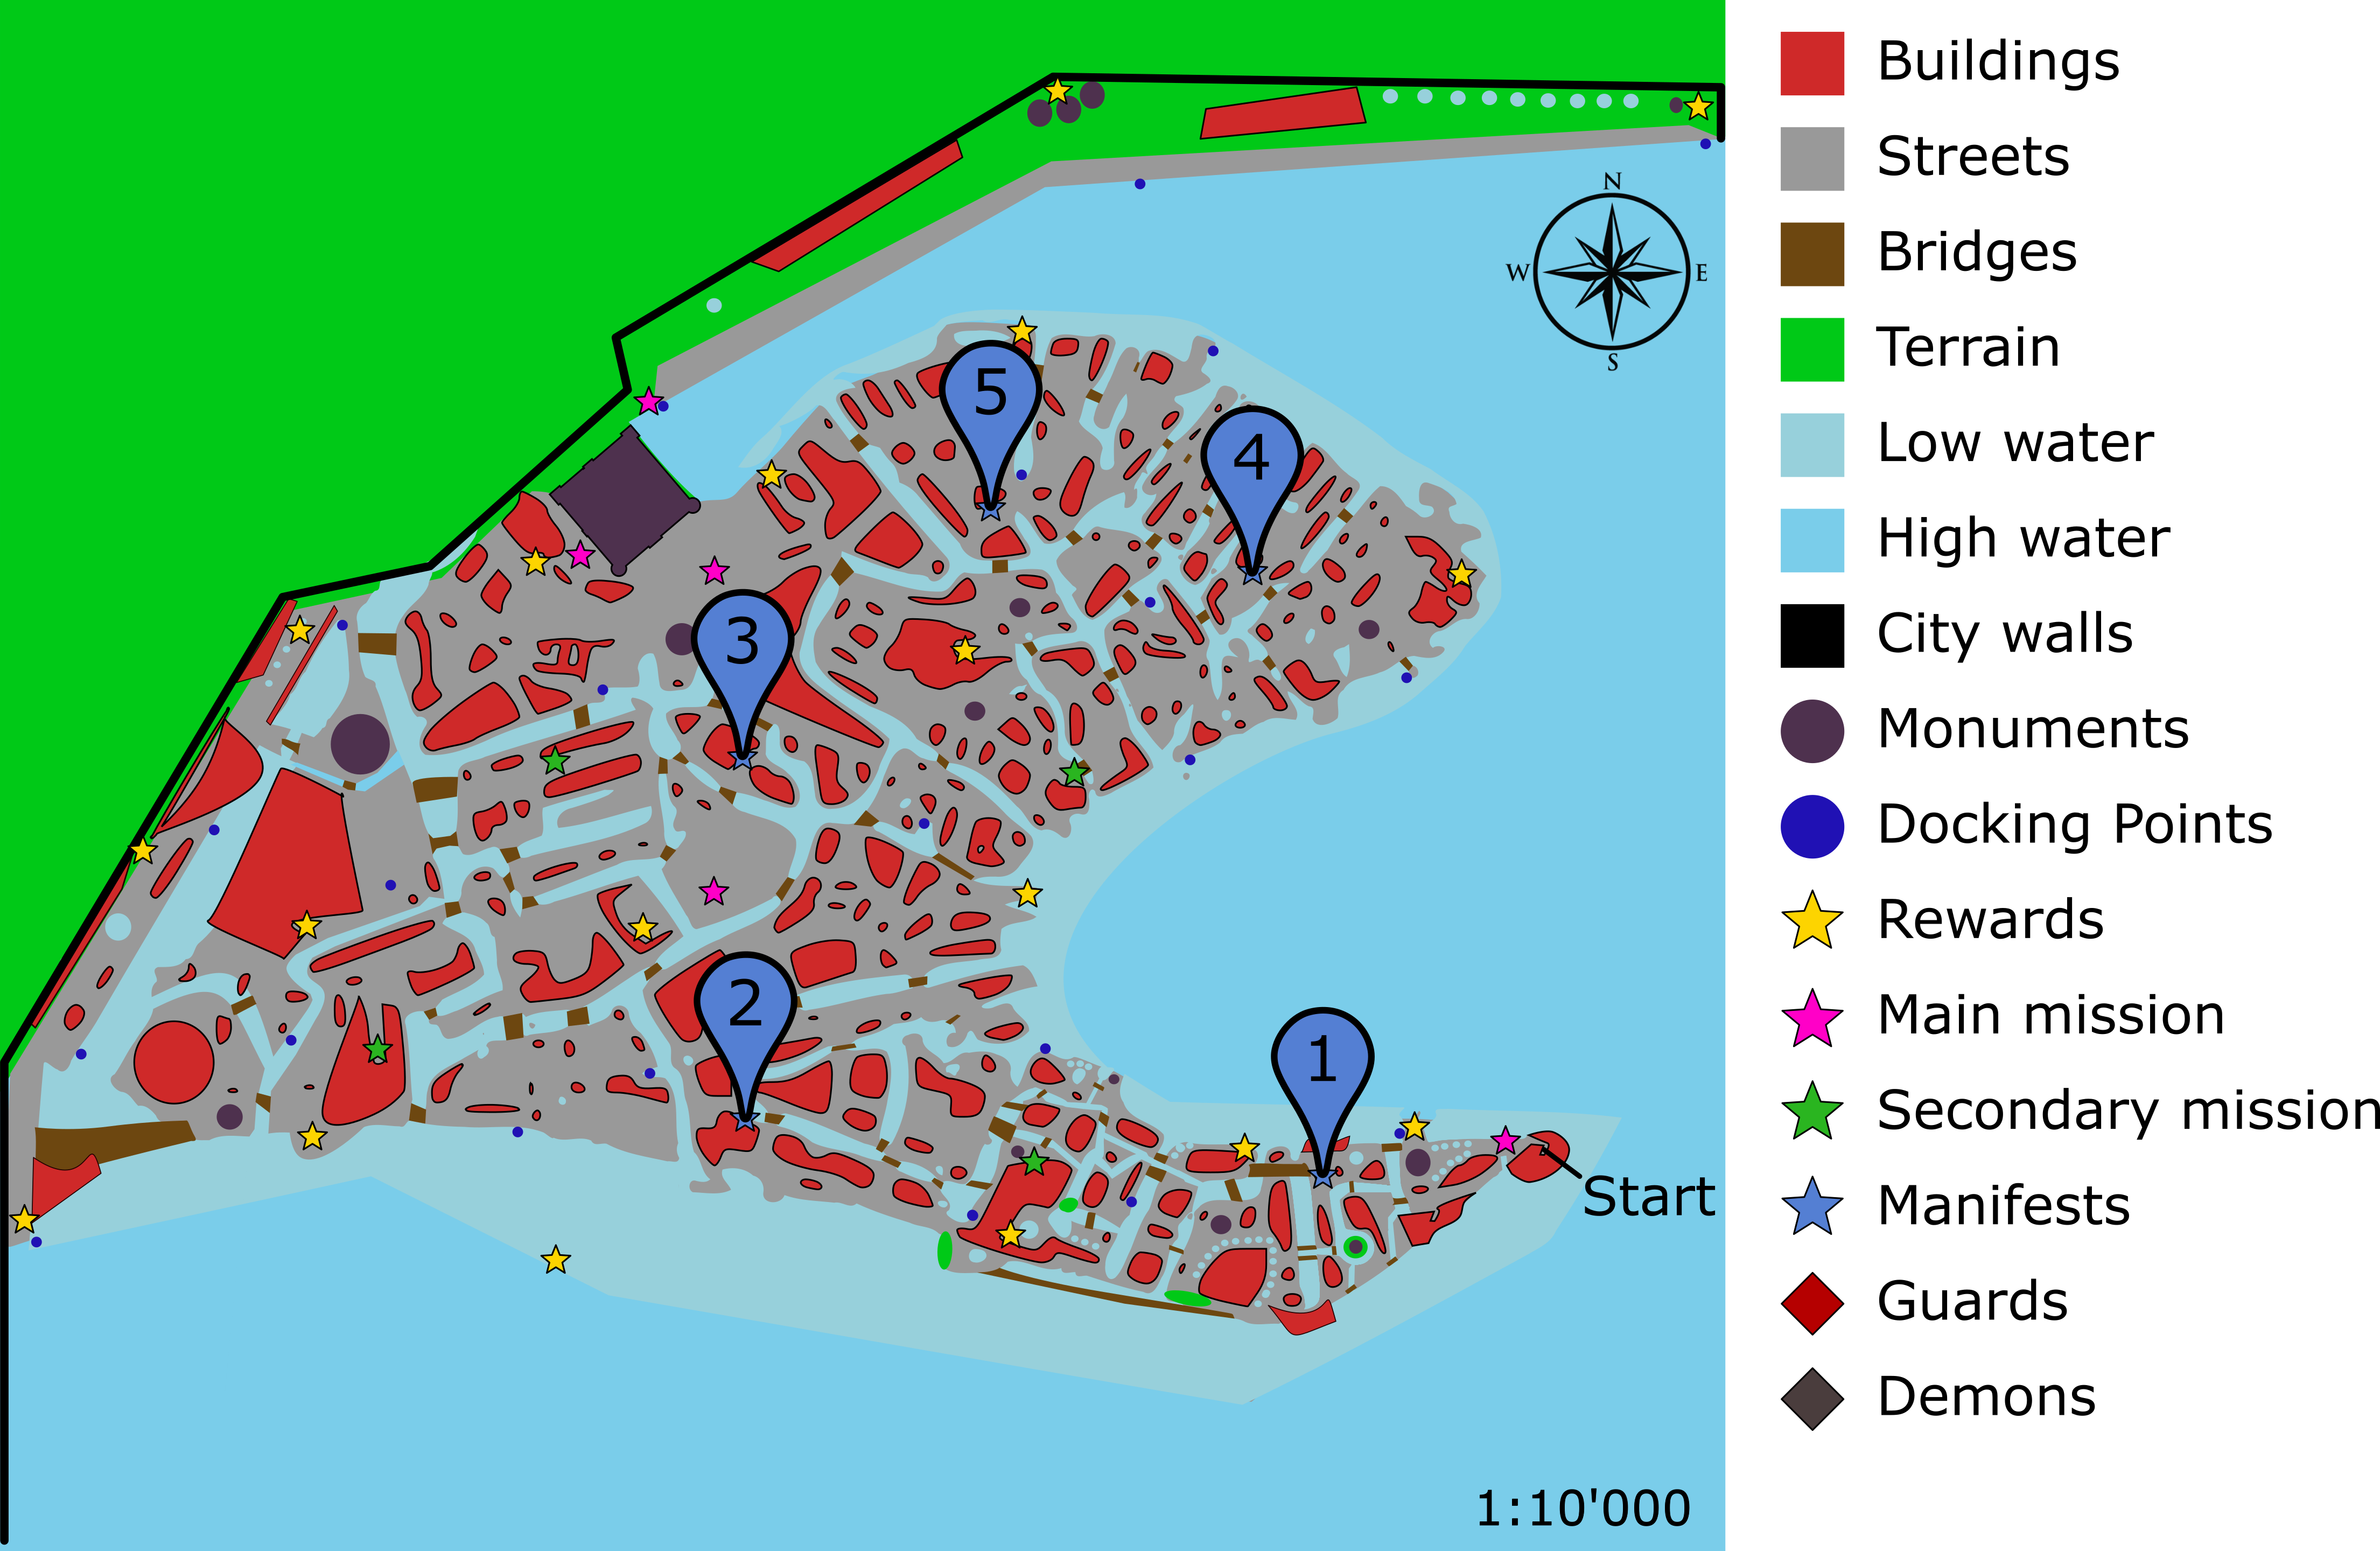
\includegraphics[width=\textwidth]{../Images/Maps/dynamiaSecondaryMissions_Manifests}
  \caption{Manifests location}
\end{figure}

\subsubsection*{Manifest \#{}1}
The manifest represents Mizar with the crown and the writing \enquote{Make Strangia great again}.

\textbf{Sophie}: Hello, manifest. Who is this woman?

\textbf{Manifest \#{}1 (solemn)}: She is our enlightened and beloved Queen regent. Thanks to her, we can make Strangia great again! Long live the Queen!

\subsubsection*{Manifest \#{}2}
The manifest represents an evil version of the King of Kingsbury and the writing \enquote{No you can't}.

\textbf{Sophie}: Hello, manifest. Who is this man?

\textbf{Manifest \#{}2 (disgusted)}: Man? He is not a man! He is the personification of evil! The king of Ingary thinks he can control us. No, you can't, king of Ingary! No, you can't!

\subsubsection*{Manifest \#{}3}
The manifest represents some soldiers with a flag of Strangia and the writing \enquote{Strangians of the world, unite!}.

\textbf{Sophie}: Hello, manifest. Who are those men?

\textbf{Manifest \#{}3 (resolute)}: This men are our beloved sons, who fight for our freedom. Ingary will not enslave us! Unite, proud sons of Dynamia! Unite, and fight for the country!

\subsubsection*{Manifest \#{}4}
The manifest represents Mizar pointing to the reader and the writing \enquote{I want you for Strangian army}.

\textbf{Sophie}: Hello, manifest. Who do you want?

\textbf{Manifest \#{}4 (proud)}: I want the strong and virtuous men of Dynamia. Fathers and sons will fight together against the enemies! Fight for your wives, fight for your sisters, fight for your daughters! Fight for Dynamia!

%The manifests represents a woman holding a baby.
%
%\textbf{Sophie}: Hello, manifest. Who is this woman?
%
%\textbf{Manifest \#{}4 (sad)}: This woman is any woman of Dynamia. Ingary has killed her husband, her child is an orphan, but she won't cry. She has to be strong for the sake of the country. Be strong, women of Dynamia!

\subsubsection*{Manifest \#{}5}
The manifest represents a flag of Strangia and the writing \enquote{Keep calm and trust the Queen}.

\textbf{Sophie}: Hello, manifest. What do you mean?

\textbf{Manifest \#{}5 (friendly)}: The Queen knows what is the best for us and how to do it. Trust the Queen, and everything will be okay.

%The manifest represents some poor people.
%
%\textbf{Sophie}: Hello, manifest. Who are these people?
%
%\textbf{Manifest \#{}5 (resolute)}: They are the future people of Dynamia if we don't stand and fight against Ingary. Ingary wants to steal our riches, but we won't let them!

\subsubsection*{After talking to all the manifests}
\textbf{Sophie (worried)}: Those manifests are all liars. Ingary wants peace for everyone.

\textbf{Calcifer (resolute)}: Don't worry, Sophie. I'm sure Howl will fix all this in a moment.

\textbf{Sophie}: You are right. Let's hurry and find him!


\subsection{Talk to all the statues}
In the city there are some statues. The player can talk to their tags in order to discover more details about the history of Strangia, in particular of Dynamia.

The statues are related to the royal family or some important historical figure.
%, such as the wizard-architect who designed the Castle of Dynamia.

The statues and their descriptions contain references to real world people or characters from other medias.

When Sophie talks to a tag, the camera rotates around its statue.

The objective is shown to the player when he/she talks to a statue for the first time.

\textbf{Reward}: the player can use the docking points as fast travel points, 150 Exp.

\begin{figure}[H]
  \centering
  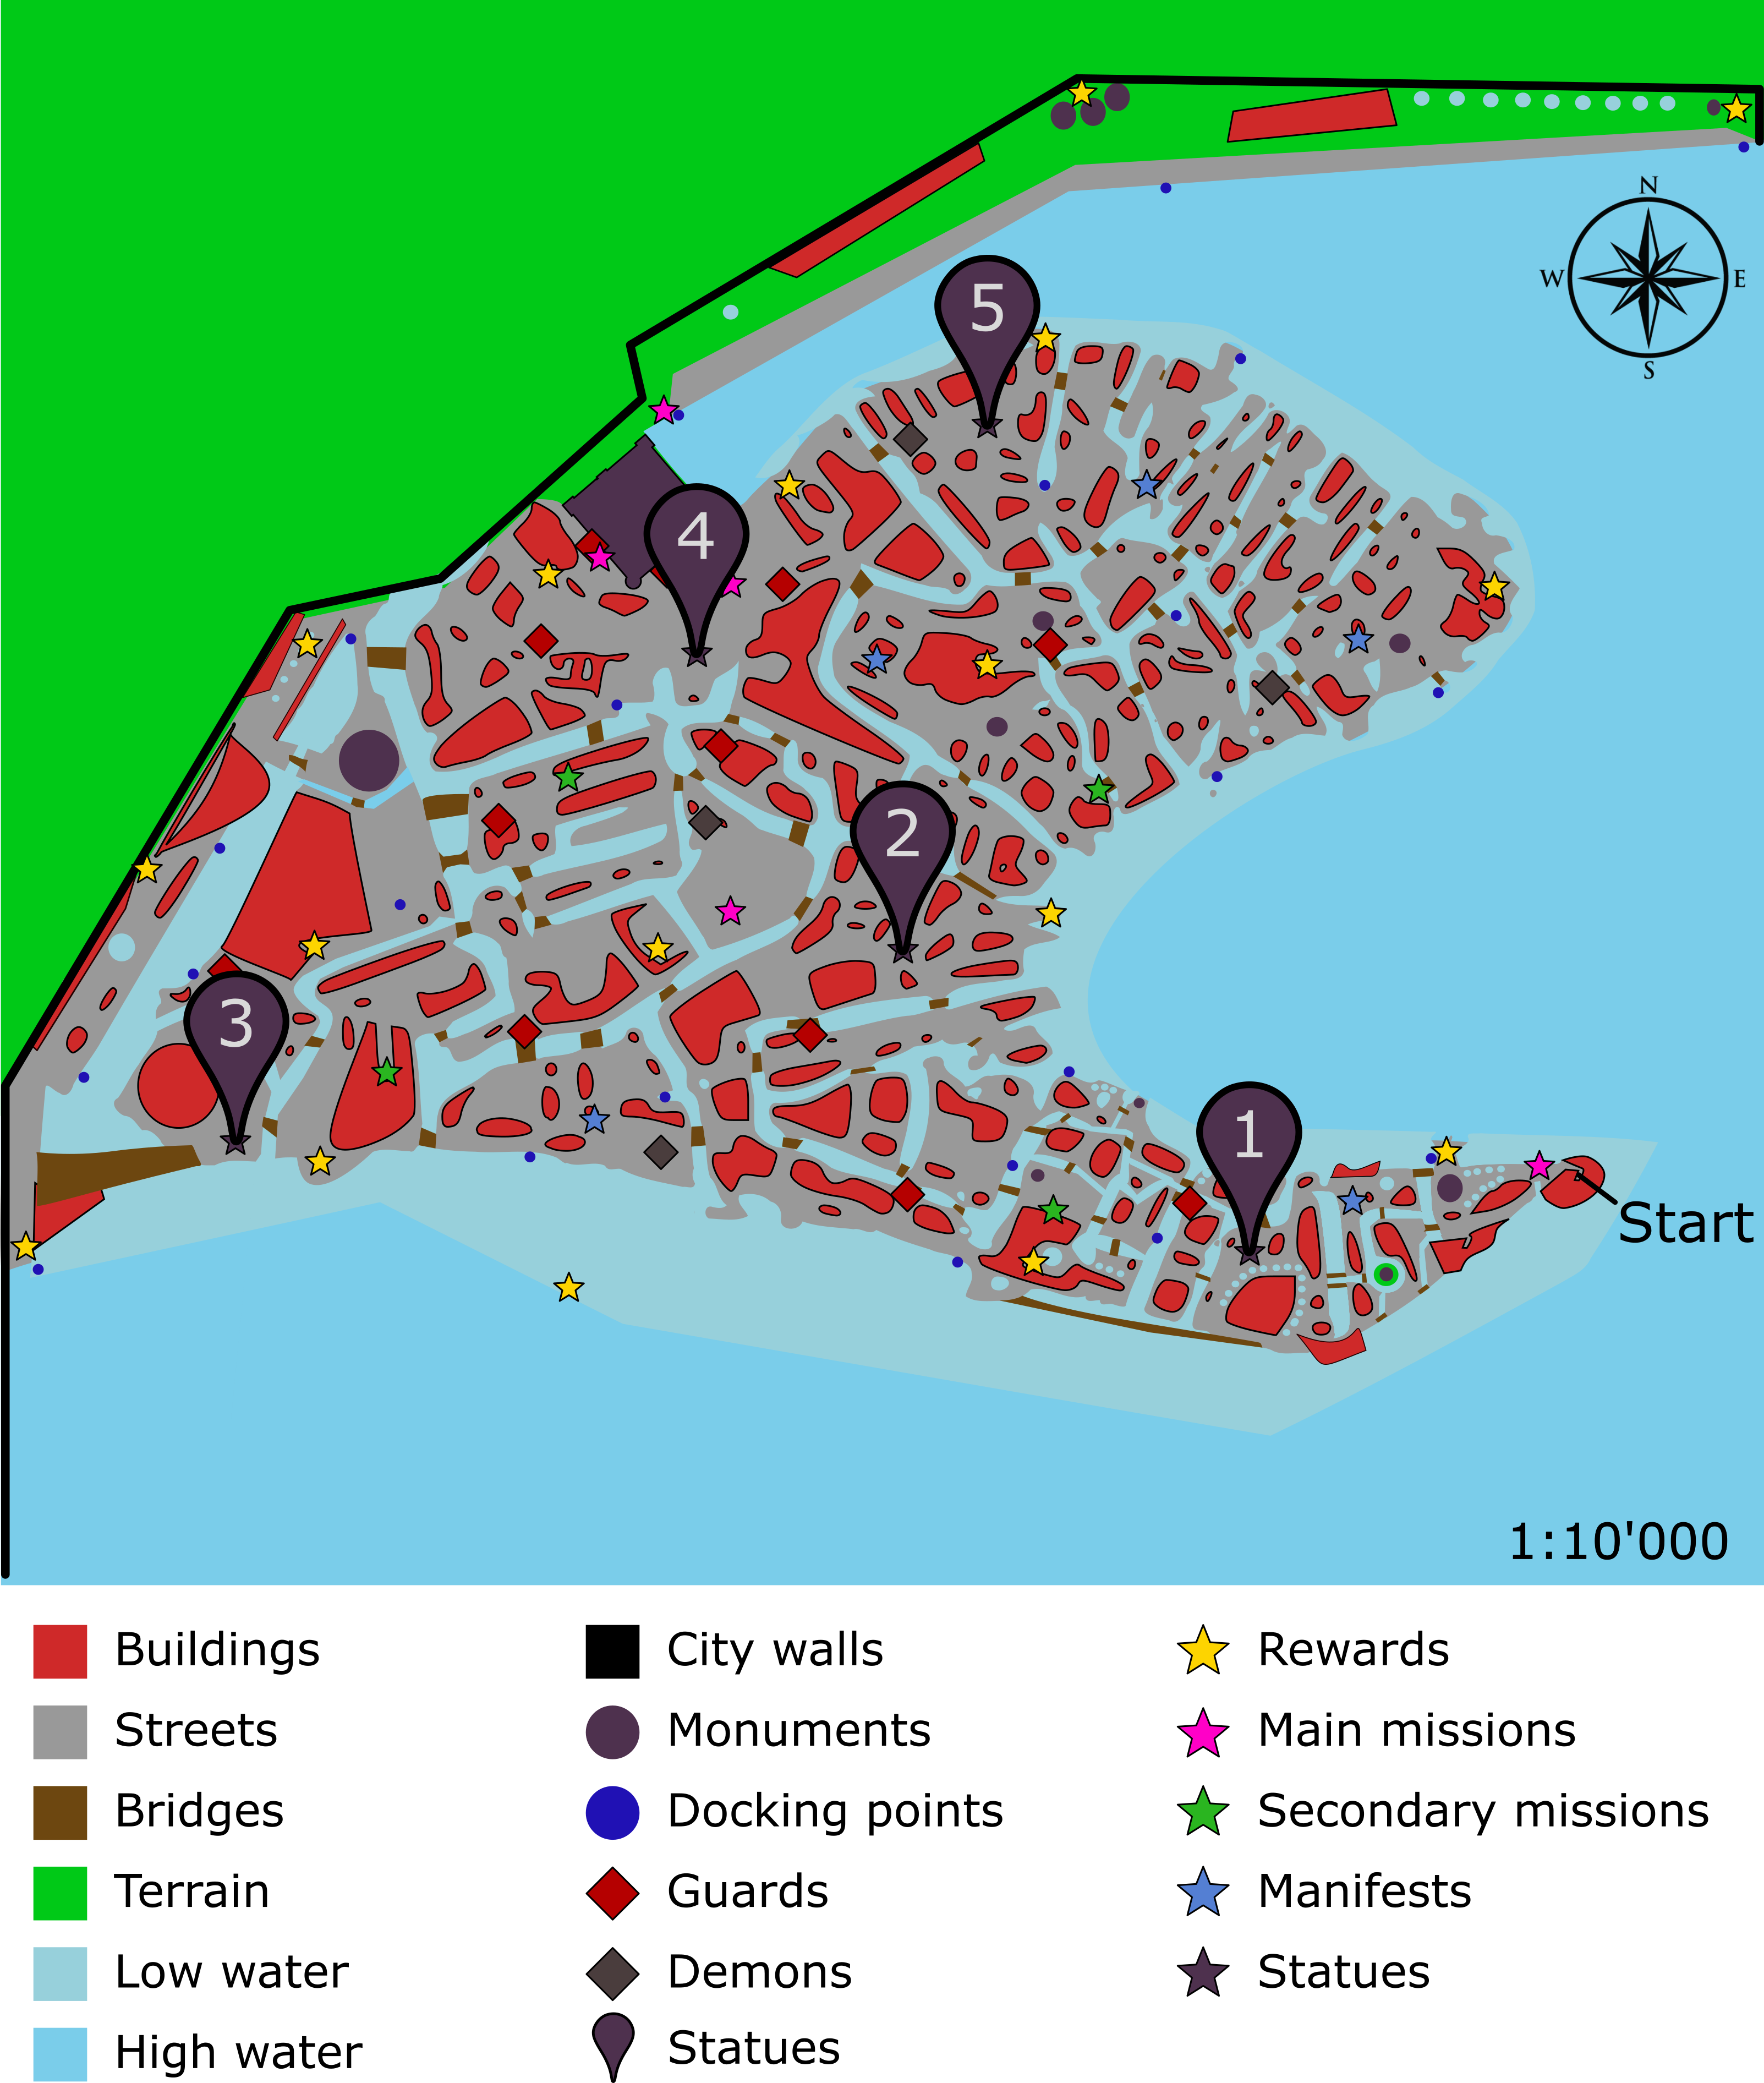
\includegraphics[width=\textwidth]{../Images/Maps/dynamiaSecondaryMissions_Statues}
  \caption{Statues location}
\end{figure}

\subsubsection*{Statue \#{}1}
The statue represents The Traveler, the first man who reached the lagoon and placed the first stone of Dynamia.

\textbf{Sophie}: Hello, statue. Who is this man?

\textbf{Statue \#{}1}: I am The Traveler*, the man who placed the first brick of Dynamia. But, hey, I'll tell you a secret: I was traveling with my crew and I wanted to go West to build my new house, but my compass didn't work properly and I ended up here and so I thought that building a house here wasn't a bad idea. Then other merchants started building their houses here too, Dynamia rose quickly and I have become a living myth.

\textbf{Sophie(laughing)}: Wow, you have been pretty lucky! Destiny* is a strange thing sometimes.

\textit{*Reference to Destiny\texttrademark and Cristoforo Colombo.}

\subsubsection*{Statue \#{}2}
The statue represents the wizard-architect who designed the Castle of Dynamia

\textbf{Sophie}: Hello, statue. Who is this man?

\textbf{Statue \#{}2}: I am the legendary wizard-architect Antonidas*. The man who designed the Castle of Dynamia centuries ago. That fortress will resist to any enemy!


\textit{*Reference to Hearthstone\texttrademark legendary card Antonidas.}

\subsubsection*{Statue \#{}3}
The statue represents a statue with red, long hair and a blindfold*: the Goddess of Fortune.

\textbf{Sophie}: Hello, statue. Who is this woman?

\textbf{Statue \#{}3}: I am the Goddess of Fortune. People of Dynamia dedicated to me even the biggest monument in the city. Merchants and fishermen ask me to help them during their impossible sea voyages, but fortune doesn't favor fools*!

\textit{*Reference to Miss Fortune, League of Legends\texttrademark{}.}

\subsubsection*{Statue \#{}4}
The statue represents the queen regent Mizar

\textbf{Sophie}: Hello, statue. Who is this woman?

\textbf{Statue \#{}4}: How can you not recognize our beloved queen regent Mizar, Defeater of Ingarians, Righteous Ruler and the Most Powerful Witch of the World? Bend your knee in front of her*!

\textit{*Reference to Game of Thrones\texttrademark{}.}

\subsubsection*{Statue \#{}5}
The statue represents a simple wizard with a necklace with a pendant made of a green shiny stone mounted on a golden circular plate*, dedicated to the wizards and soldiers who died during the wars.

\textbf{Sophie}: Hello, statue. Who is this man?

\textbf{Statue \#{}5}: This is the statue of the Unknown Wizard. This is dedicated to every soldier and wizard who died during the wars of Strangia. I hope Strangia will ask to Ingary to bargain*, so this massacre will end!

\textit{*Reference to Marvel\texttrademark 's Doctor Strange.}

\subsubsection*{After talking to all the Statues}
\textbf{Sophie}: I have a feeling of dejà vu. I have seen all this statues somewhere else...


\subsection{Help the doctor}
Find 10 blue seaweeds, that grow on the wooden stakes of the docking points. On each docking point there are 3 or 4 blue seaweeds (50\% chance for both of them, 85\% chance for collecting the required blue seaweed visiting 3 docking points).

The player can find the doctor because there are several people who move around his medical office talking about how busy he is.

The player can visit only the hall of the medical office, that is quite messy because there are a lot of patients, so the nurses has prepared some makeshift beds in the hall. There are some locked doors with the writing "AUTHORIZED PERSONNEL ONLY".

The doctor is an old man with gray hair and mustaches. He wears a white gown and has a stethoscope. His clothes are quite old and worn-out.

\textbf{Reward}: nurse hat, 150 Exp.

\begin{figure}[H]
  \centering
  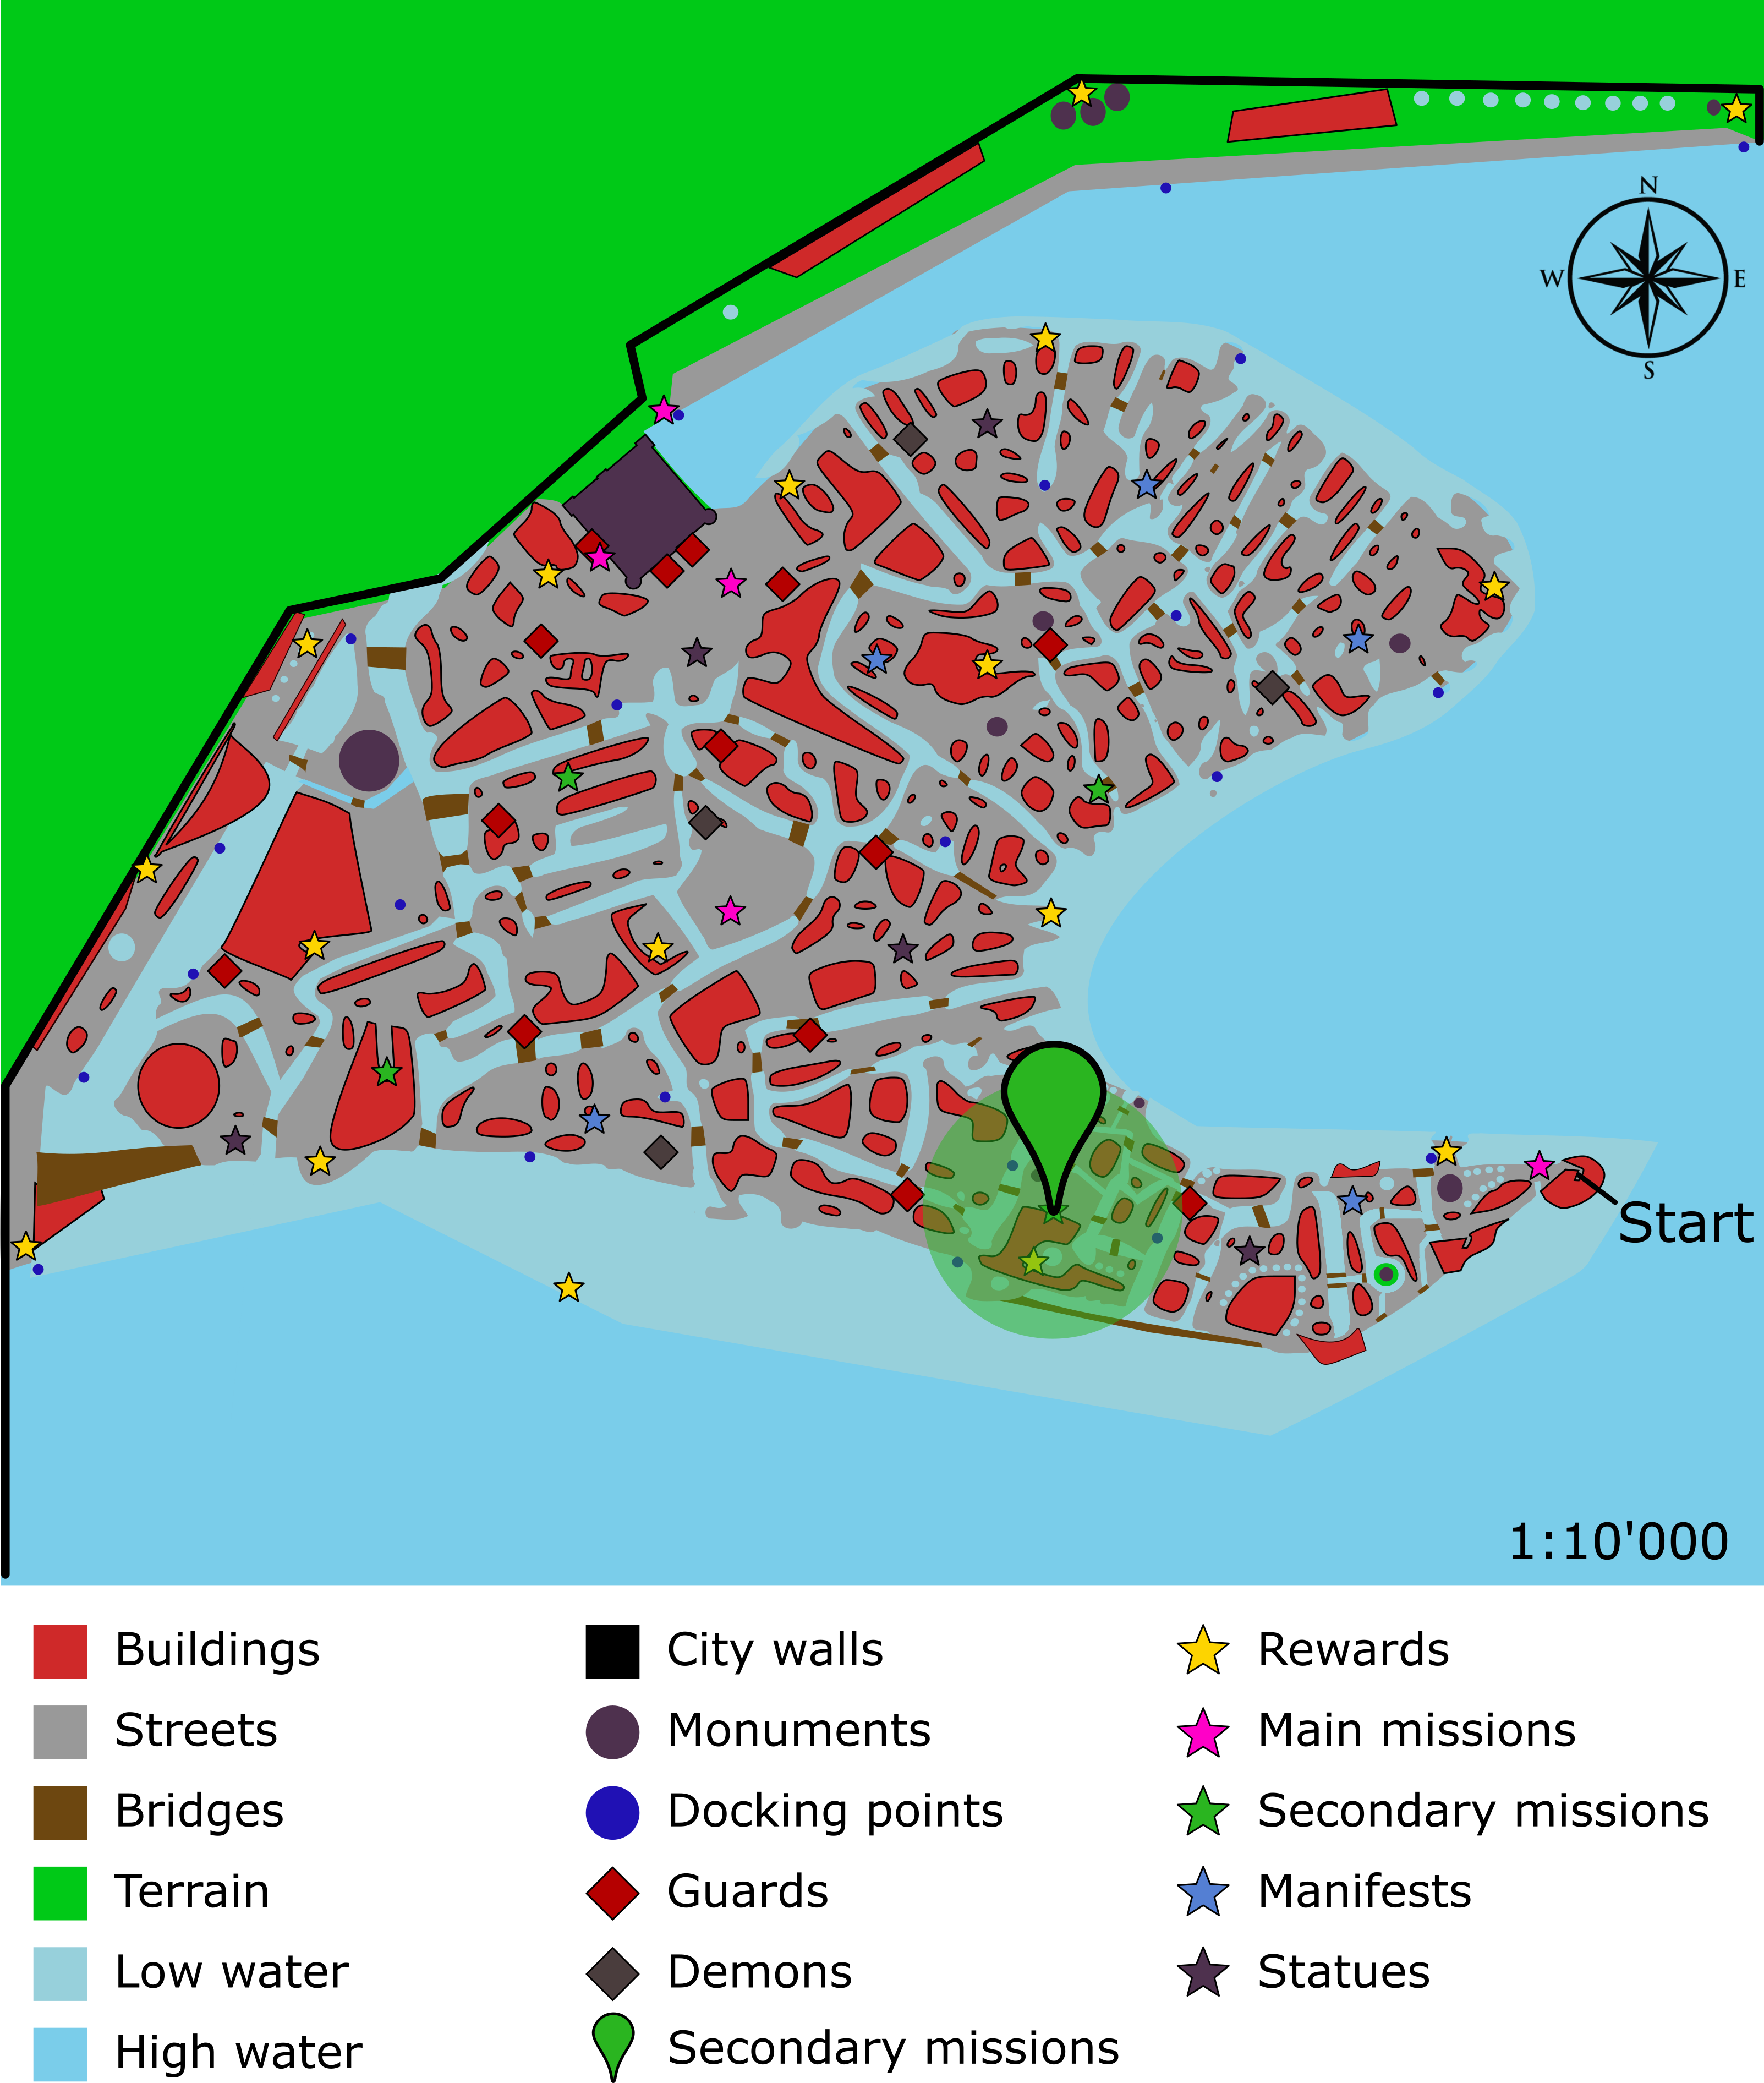
\includegraphics[width=\textwidth]{../Images/Maps/dynamiaSecondaryMissions_Doctor}
  \caption{Secondary mission initial location and activation area}
\end{figure}

\begin{figure}[H]
  \centering
  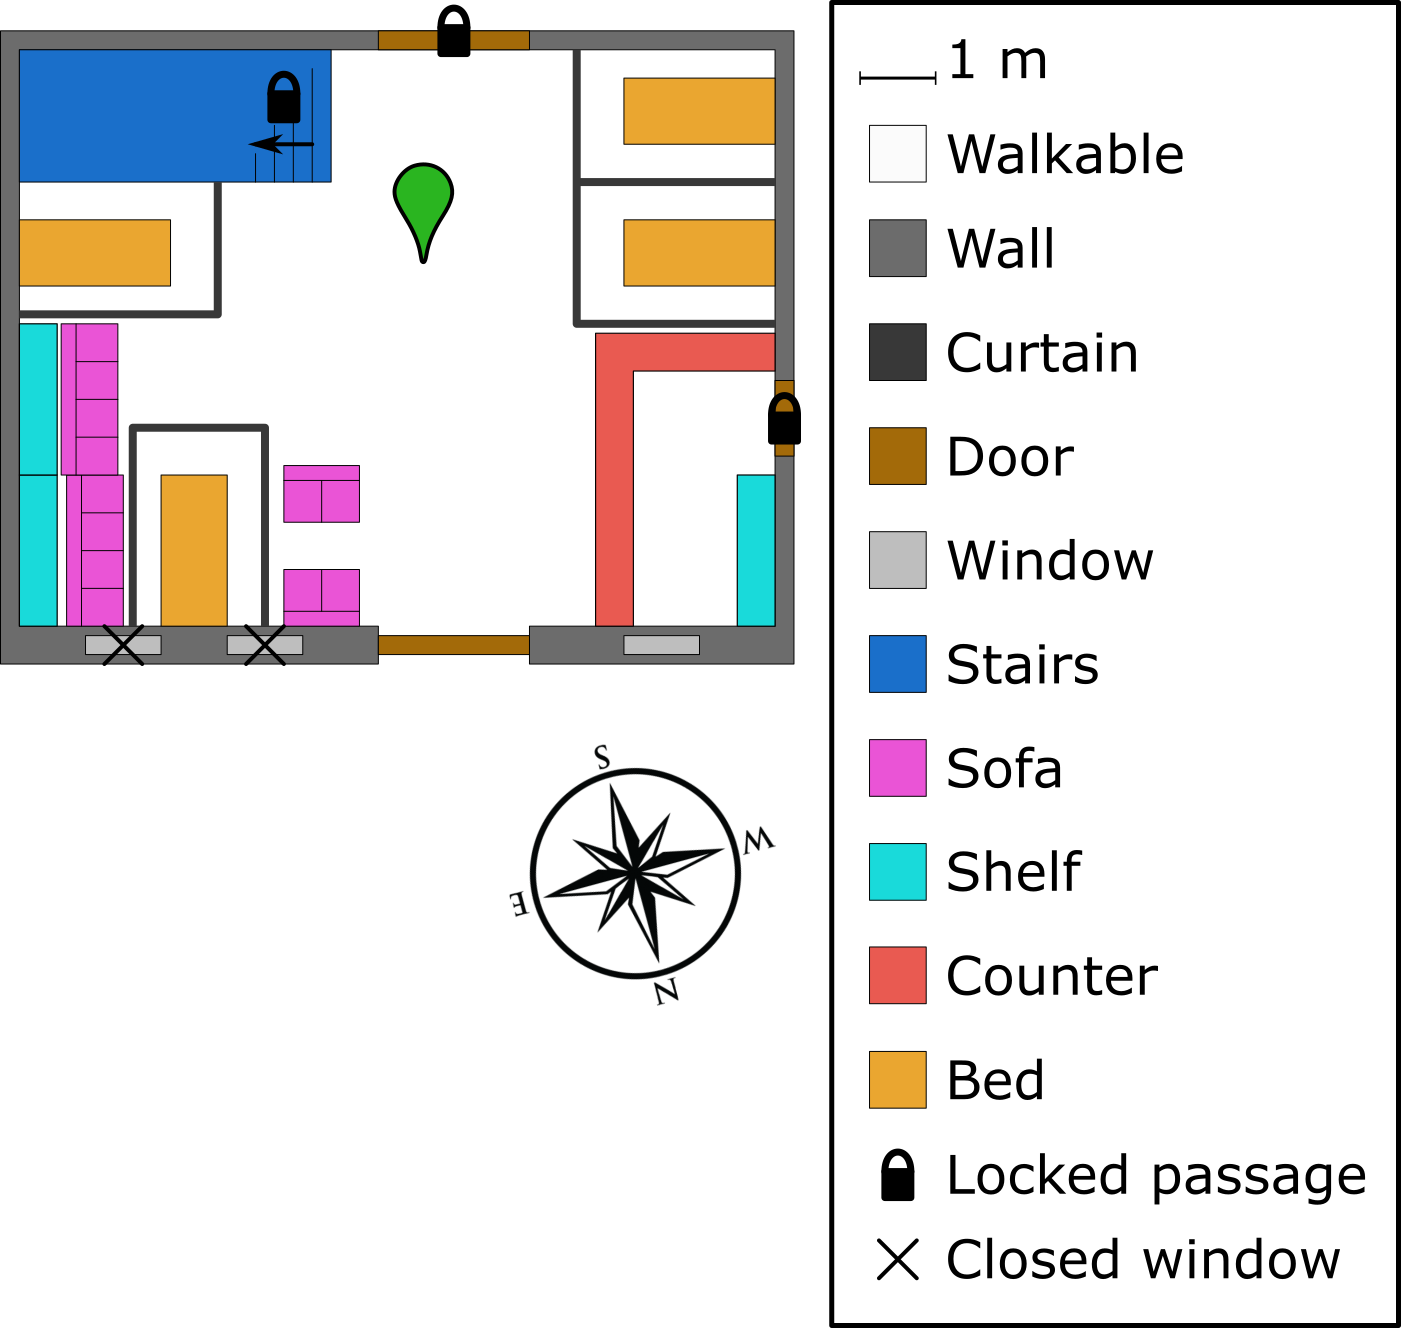
\includegraphics[width=\textwidth]{../Images/Maps/medicalOffice}
  \caption{Medical office and doctor location}
\end{figure}

\begin{figure}[H]
  \centering
  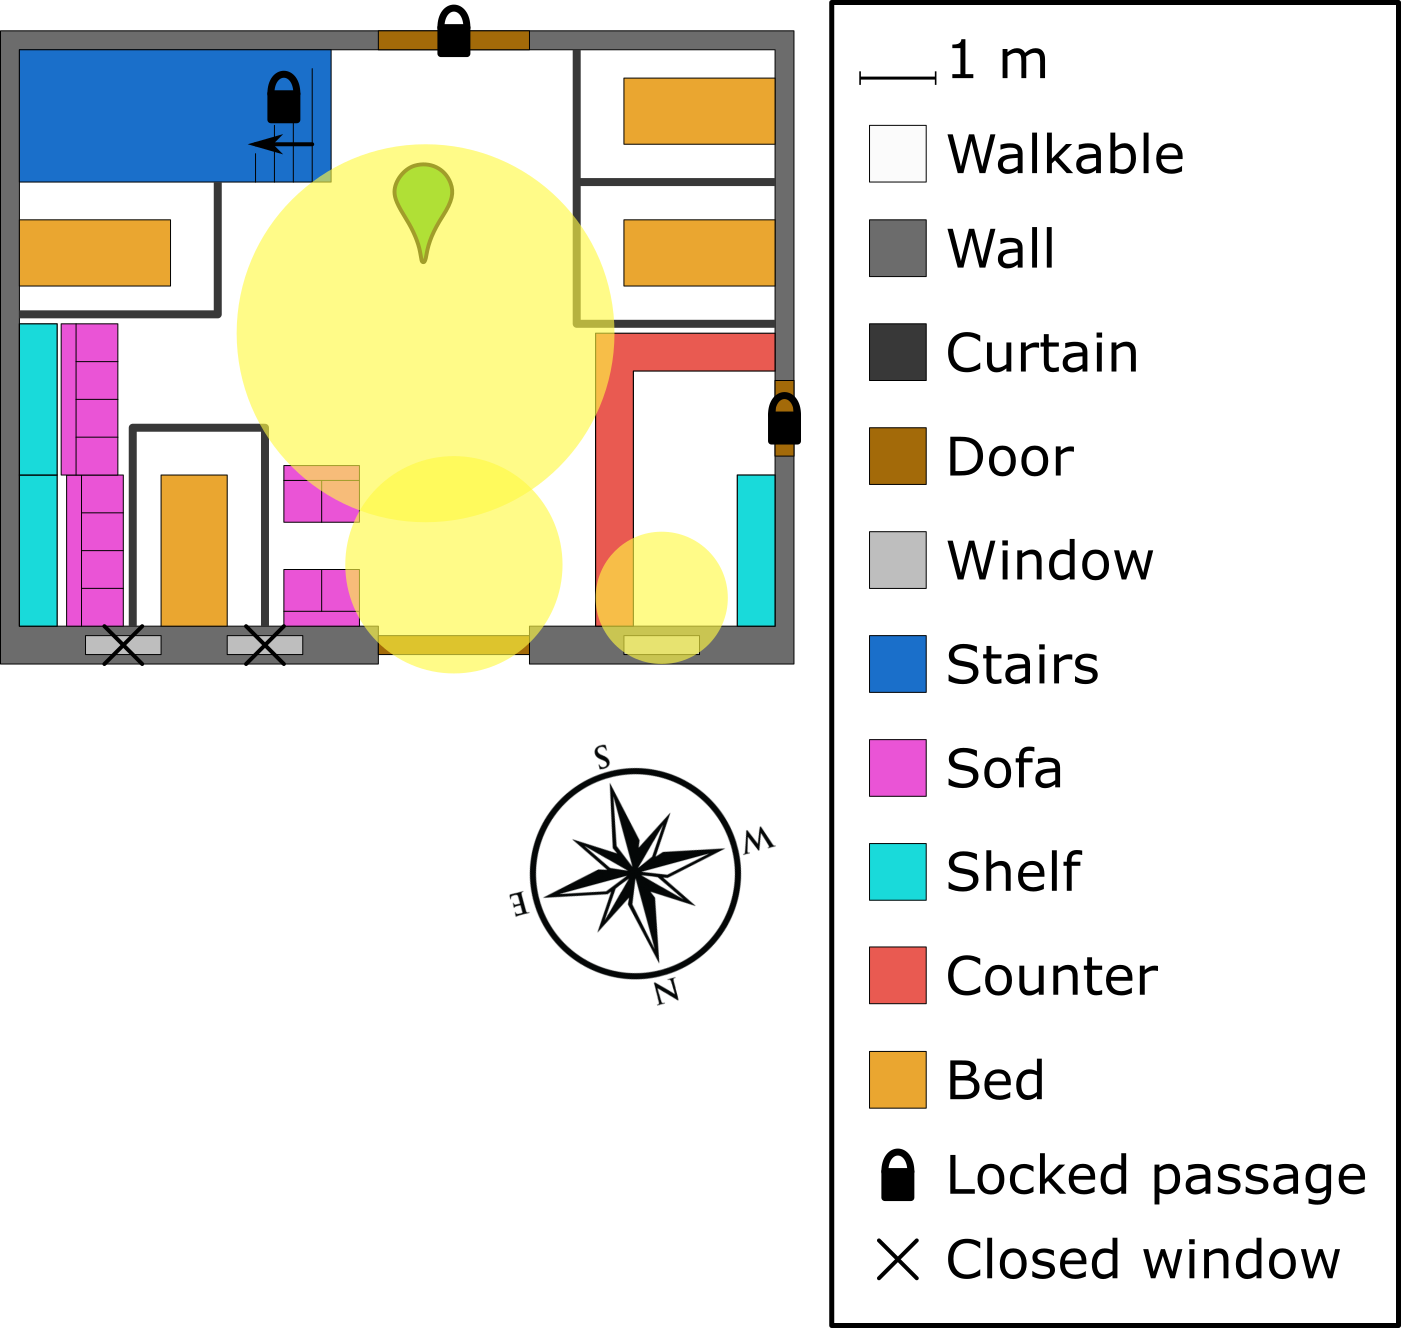
\includegraphics[width=\textwidth]{../Images/Maps/medicalOfficeLighting}
  \caption{Medical office lighting}
\end{figure}

\subsubsection*{Starting mission cutscene}
\begin{screenplay}
\extslug[afternoon]{Dynamia, southern area}

The doctor, a quite old man, is reading some papers. He is worried.

\begin{dialogue}[to himself]{Doctor}
The blue seaweed is almost over. If only there were my assistants...
\end{dialogue}

\begin{dialogue}{Sophie}
Excuse me, doctor. I heard that you need some help.
\end{dialogue}

\begin{dialogue}{Doctor}
Unfortunately, I do. I have a lot of patients that suffer from blue fever. Also our king, may he rest in peace, had suffered form severe blue fever. They need the extract of blue seaweed, but I have no time to collect enough seaweed and all my apprentices have gone to war.
\end{dialogue}

\begin{dialogue}{Sophie}
I can take some for you. Where can I find it?
\end{dialogue}

\begin{dialogue}{Doctor}
Oh, it very simple: it grows on the wooden stakes of the docking points. Bring me some if you have time.
\end{dialogue}

\end{screenplay}

\subsubsection*{NPC's lines during the mission}
\textbf{Doctor (busy)}: The blue seaweed grows on the wooden stakes of the docking points. If you can bring me some, that would be great for my patients.

\subsubsection*{Ending mission cutscene}
\begin{screenplay}
\extslug[afternoon]{Dynamia, southern area}

\begin{dialogue}{Sophie}
Doctor, I take some blue seaweed. I hope it is enough.
\end{dialogue}

\begin{dialogue}{Doctor}
Oh, thanks a lot! I'll immediately start making some extract. And, please, let me give you this hat. In recognition of your efforts.
\end{dialogue}

The doctor gives Sophie the reward.

\end{screenplay}

\subsubsection*{NPC's lines after the mission}
\textbf{Doctor}: Thanks to you my patients are getting better. I wish we have more people like you.


\subsection{Help the traitor guard}
Find the traitor guard's hat and bring it to him. The hat is in a guarded warehouse, so the player has to use Calcifer to enter through an open window. In order to do that, Sophie has to jump on the box under the window.

The player can recognize the guard because he is sitting at a small table and he is drinking, complaining himself and shaking his head.

Calcifer can jump on 0,5-meters-tall objects. The small boxes are 0.5-meters-tall. The standard boxes are 1-meter-tall. The boxes with barrel are 2-meters-tall. In order to exit the warehouse, the player has to push some boxes to create a stair and reach the open window (see the Height view in \textit{Figure 7.20}). Calcifer cannot push the boxes with barrel and cannot pull any box.

The guard is a 25-years-old man, he has short black hair and no beard. He is thin and not very tall.

\textbf{Reward}: map of the castle, 150 Exp.

\begin{figure}[H]
  \centering
  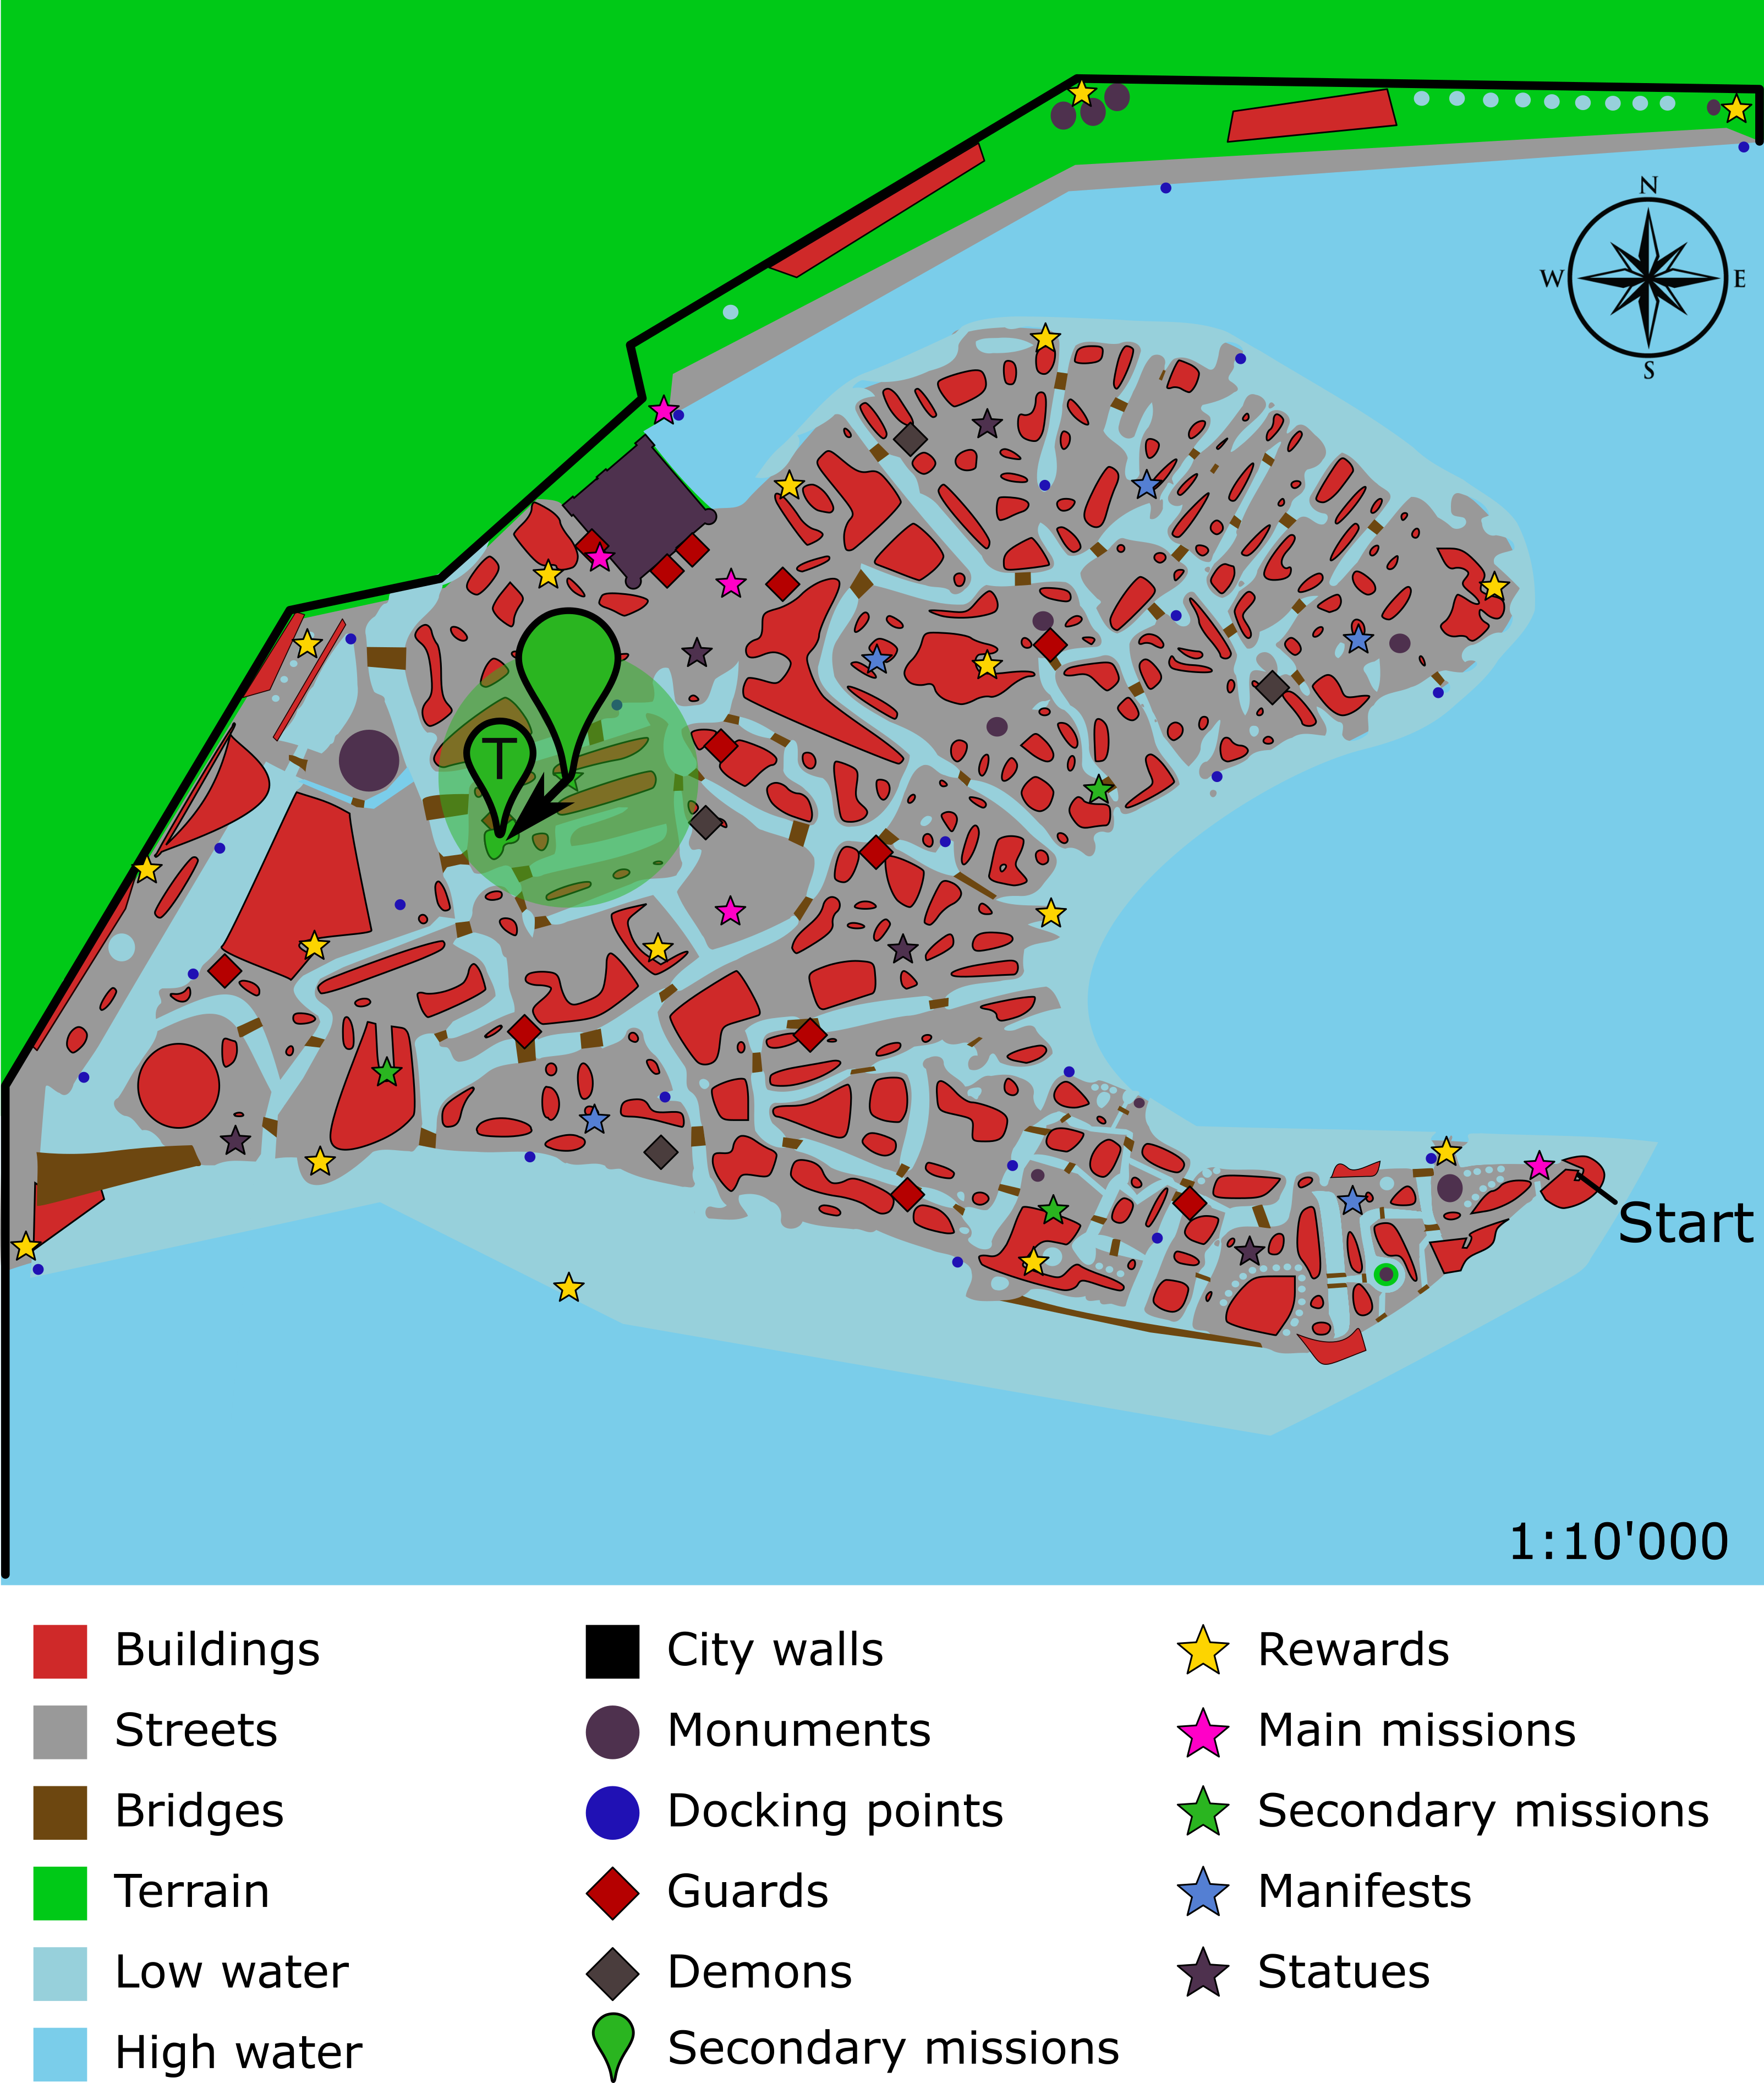
\includegraphics[width=\textwidth]{../Images/Maps/dynamiaSecondaryMissions_Guard}
  \caption{Secondary mission initial location, activation area and target storage (T)}
\end{figure}

\begin{figure}[H]
  \centering
  \includegraphics[width=\textwidth]{../Images/Maps/warehouse}
  \caption{Warehouse, open window location (gray) and hat location (green)}
\end{figure}

\begin{figure}[H]
  \centering
  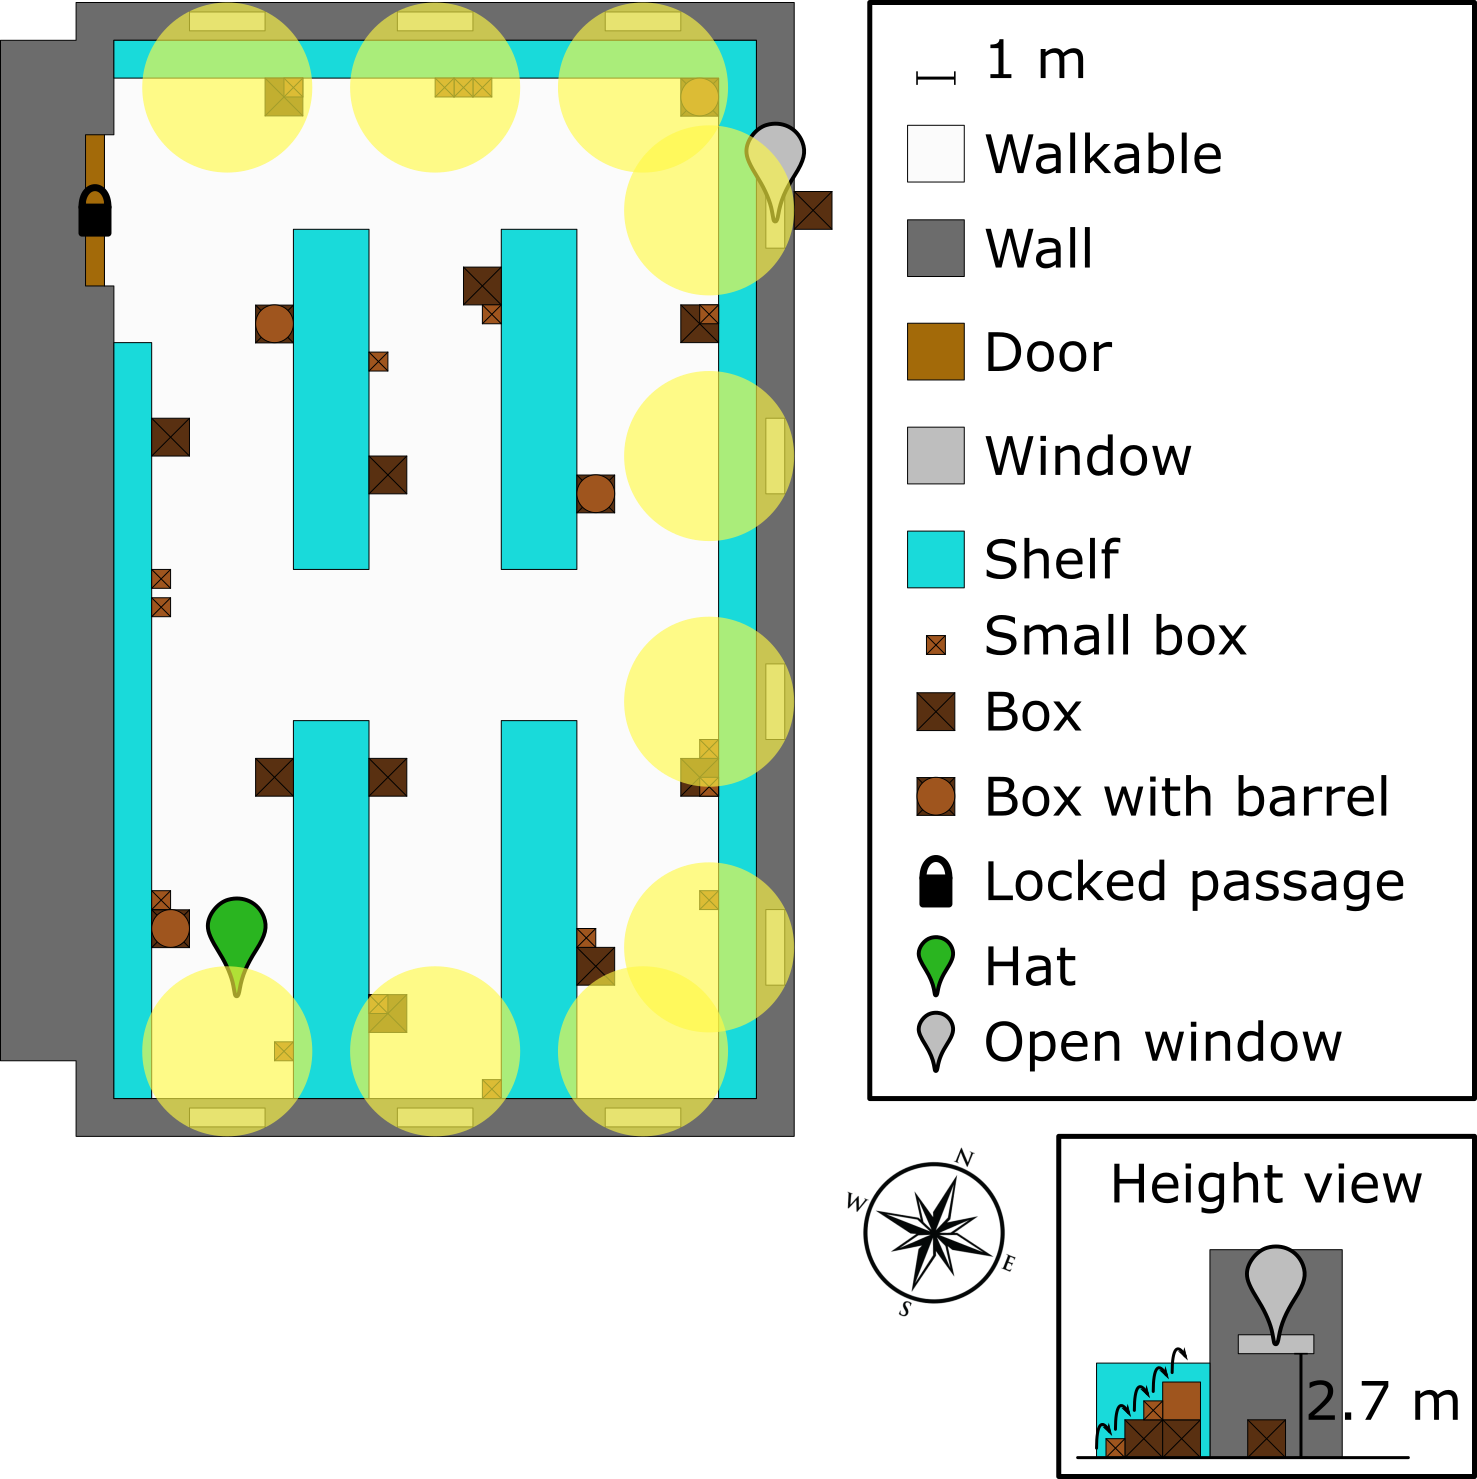
\includegraphics[width=\textwidth]{../Images/Maps/warehouseLighting}
  \caption{Warehouse lighting}
\end{figure}

\begin{figure}[H]
  \centering
  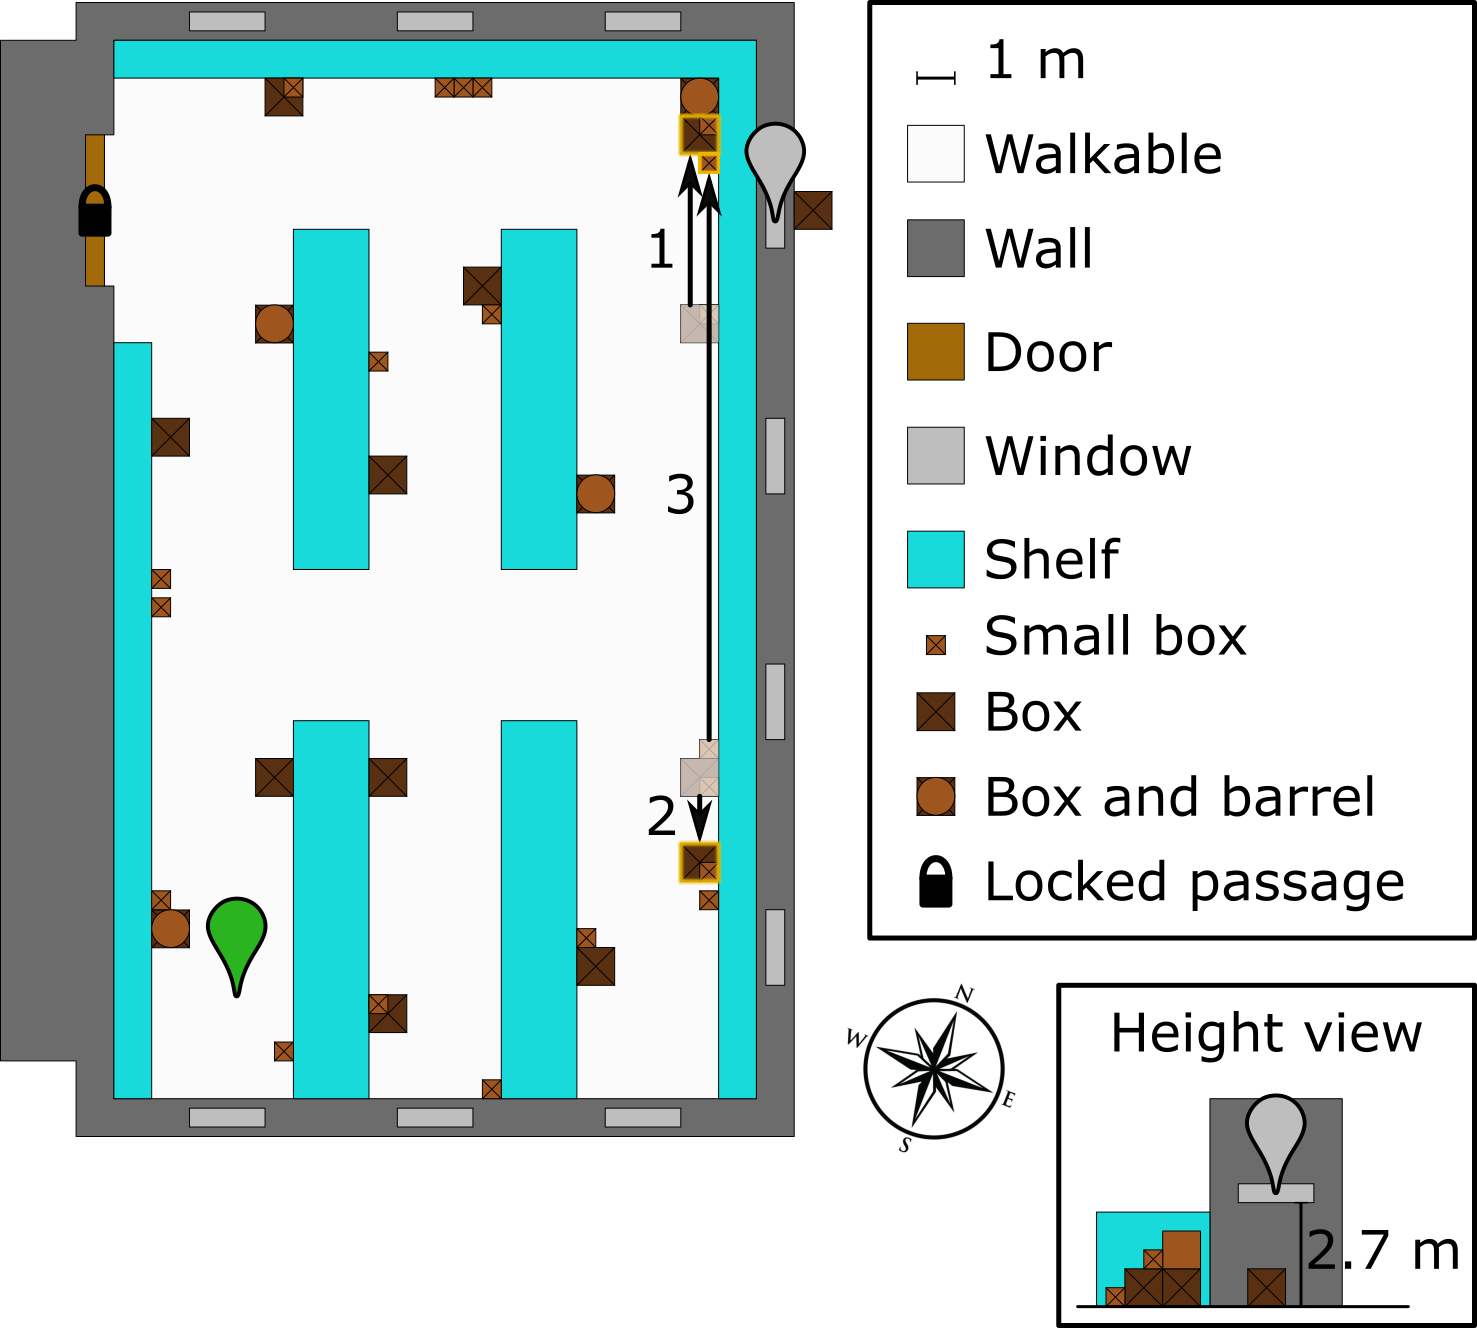
\includegraphics[width=14cm]{../Images/Maps/warehouseSolution}
  \caption{Possible solution for the environmental puzzle}
\end{figure}

\begin{figure}[H]
  \centering
  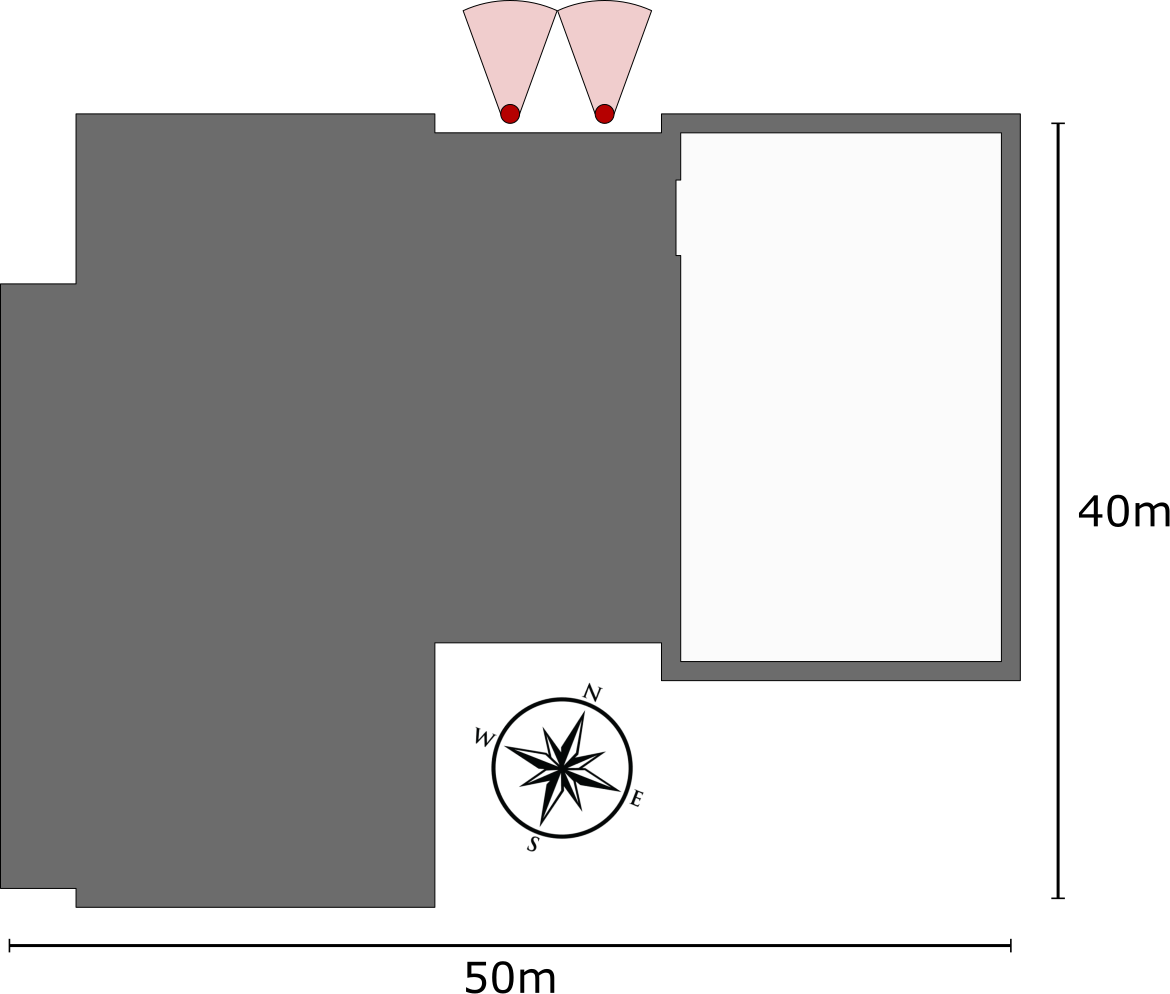
\includegraphics[width=12cm]{../Images/Maps/warehouseBuilding}
  \caption{Warehouse building}
\end{figure}

\subsubsection*{Starting mission cutscene}
\begin{screenplay}
\extslug[afternoon]{Dynamia, central area}

\begin{dialogue}[forlorn]{Traitor guard}
Oh, I'm done. If they find it, I'm dead.
\end{dialogue}

\begin{dialogue}{Sophie}
Excuse me, what's the problem?
\end{dialogue}

\begin{dialogue}[forlorn]{Traitor guard}
Mmh? Oh, none of your concern. Just leave me alone.
\end{dialogue}

\begin{dialogue}{Sophie}
If you need help, maybe I can help you.
\end{dialogue}

\begin{dialogue}[surprised]{Calcifer}
You what?!
\end{dialogue}

\begin{dialogue}[forlorn]{Traitor guard}
I'm sure you won't fail the queen.
\end{dialogue}

\begin{dialogue}{Sophie}
I'm in trouble too and I'm not a subject of the queen. If I can help you, I'll do it.
\end{dialogue}

\begin{dialogue}[weird]{Traitor guard}
Ok. Fine. Do you see that big storage?
\end{dialogue}

The camera shows a nearby building with an open window.

\begin{dialogue}[continuing]{Traitor guard}
My hat is in there. If you can bring it to me without being detected by the guards, you'll save my life.
\end{dialogue}

\begin{dialogue}{Sophie}
Ok, just wait me there.
\end{dialogue}

Sophie steps away from the guard.

\begin{dialogue}[disappointed]{Calcifer}
Do you really wanna help a guard?!
\end{dialogue}

\begin{dialogue}{Sophie}
Maybe he's in trouble for a good reason. If we help him, maybe he'll help us.
\end{dialogue}

\end{screenplay}

\subsubsection*{NPC's lines during the mission}
\textbf{Traitor guard (forlorn)}: My hat is in that storage. I wonder how long will it take for the other guards to find it.

\subsubsection*{Ending mission cutscene}
\begin{screenplay}
\extslug[afternoon]{Dynamia, central area}

Sophie pulls the hat to the traitor guard.

\begin{dialogue}{Sophie}
Hey, here is your hat.
\end{dialogue}

The traitor guard gets up surprised and takes the hat. He observes it very carefully.

\begin{dialogue}[surprised]{Traitor guard}
It's it! It's really my hat! You saved my life!
\end{dialogue}

\begin{dialogue}{Sophie}
But why is it so important?
\end{dialogue}

\begin{dialogue}[serious]{Traitor guard}
Well, I think I can tell you. I robbed some foods and I gave it to some people of the ghetto. I know it's wrong to rob, but life is very hard for them nowadays. Now, how can I repay you?
\end{dialogue}

\begin{dialogue}{Sophie}
Well, maybe you heard about a wizard called Howl? I'm looking for him.
\end{dialogue}

\begin{dialogue}[thinking]{Traitor guard}
Howl... No, I'm sorry. But I heard some guards from the castle talking about a wizard. Wait, this might help you.
\end{dialogue}

The guard gives Sophie a map of the castle.

\begin{dialogue}[continuing]{Traitor guard}
Now I have to go. Thank you very much and I hope you'll find your Howl!
\end{dialogue}

The guard runs away.

\end{screenplay}


\subsection{Rebuild the bridge}
Use Calcifer's ability to build a new bridge using some debris found nearby the location of the mission.

Within a range of 200 meters from the collapsed bridge there are many small piles of debris, the player has to collect 5 of them to rebuild the bridge.

The player can find the mission because there are many NPCs nearby the collapsed bridge who points to it or are trying to rebuild it. The group is lead by a dark skinned tall woman. She wears a very worn out blouse and work gloves. She has an old belt with many tools.

\textbf{Reward}: 15\% discount on every crafting material in Dynamia, 150 Exp.

\begin{figure}[H]
  \centering
  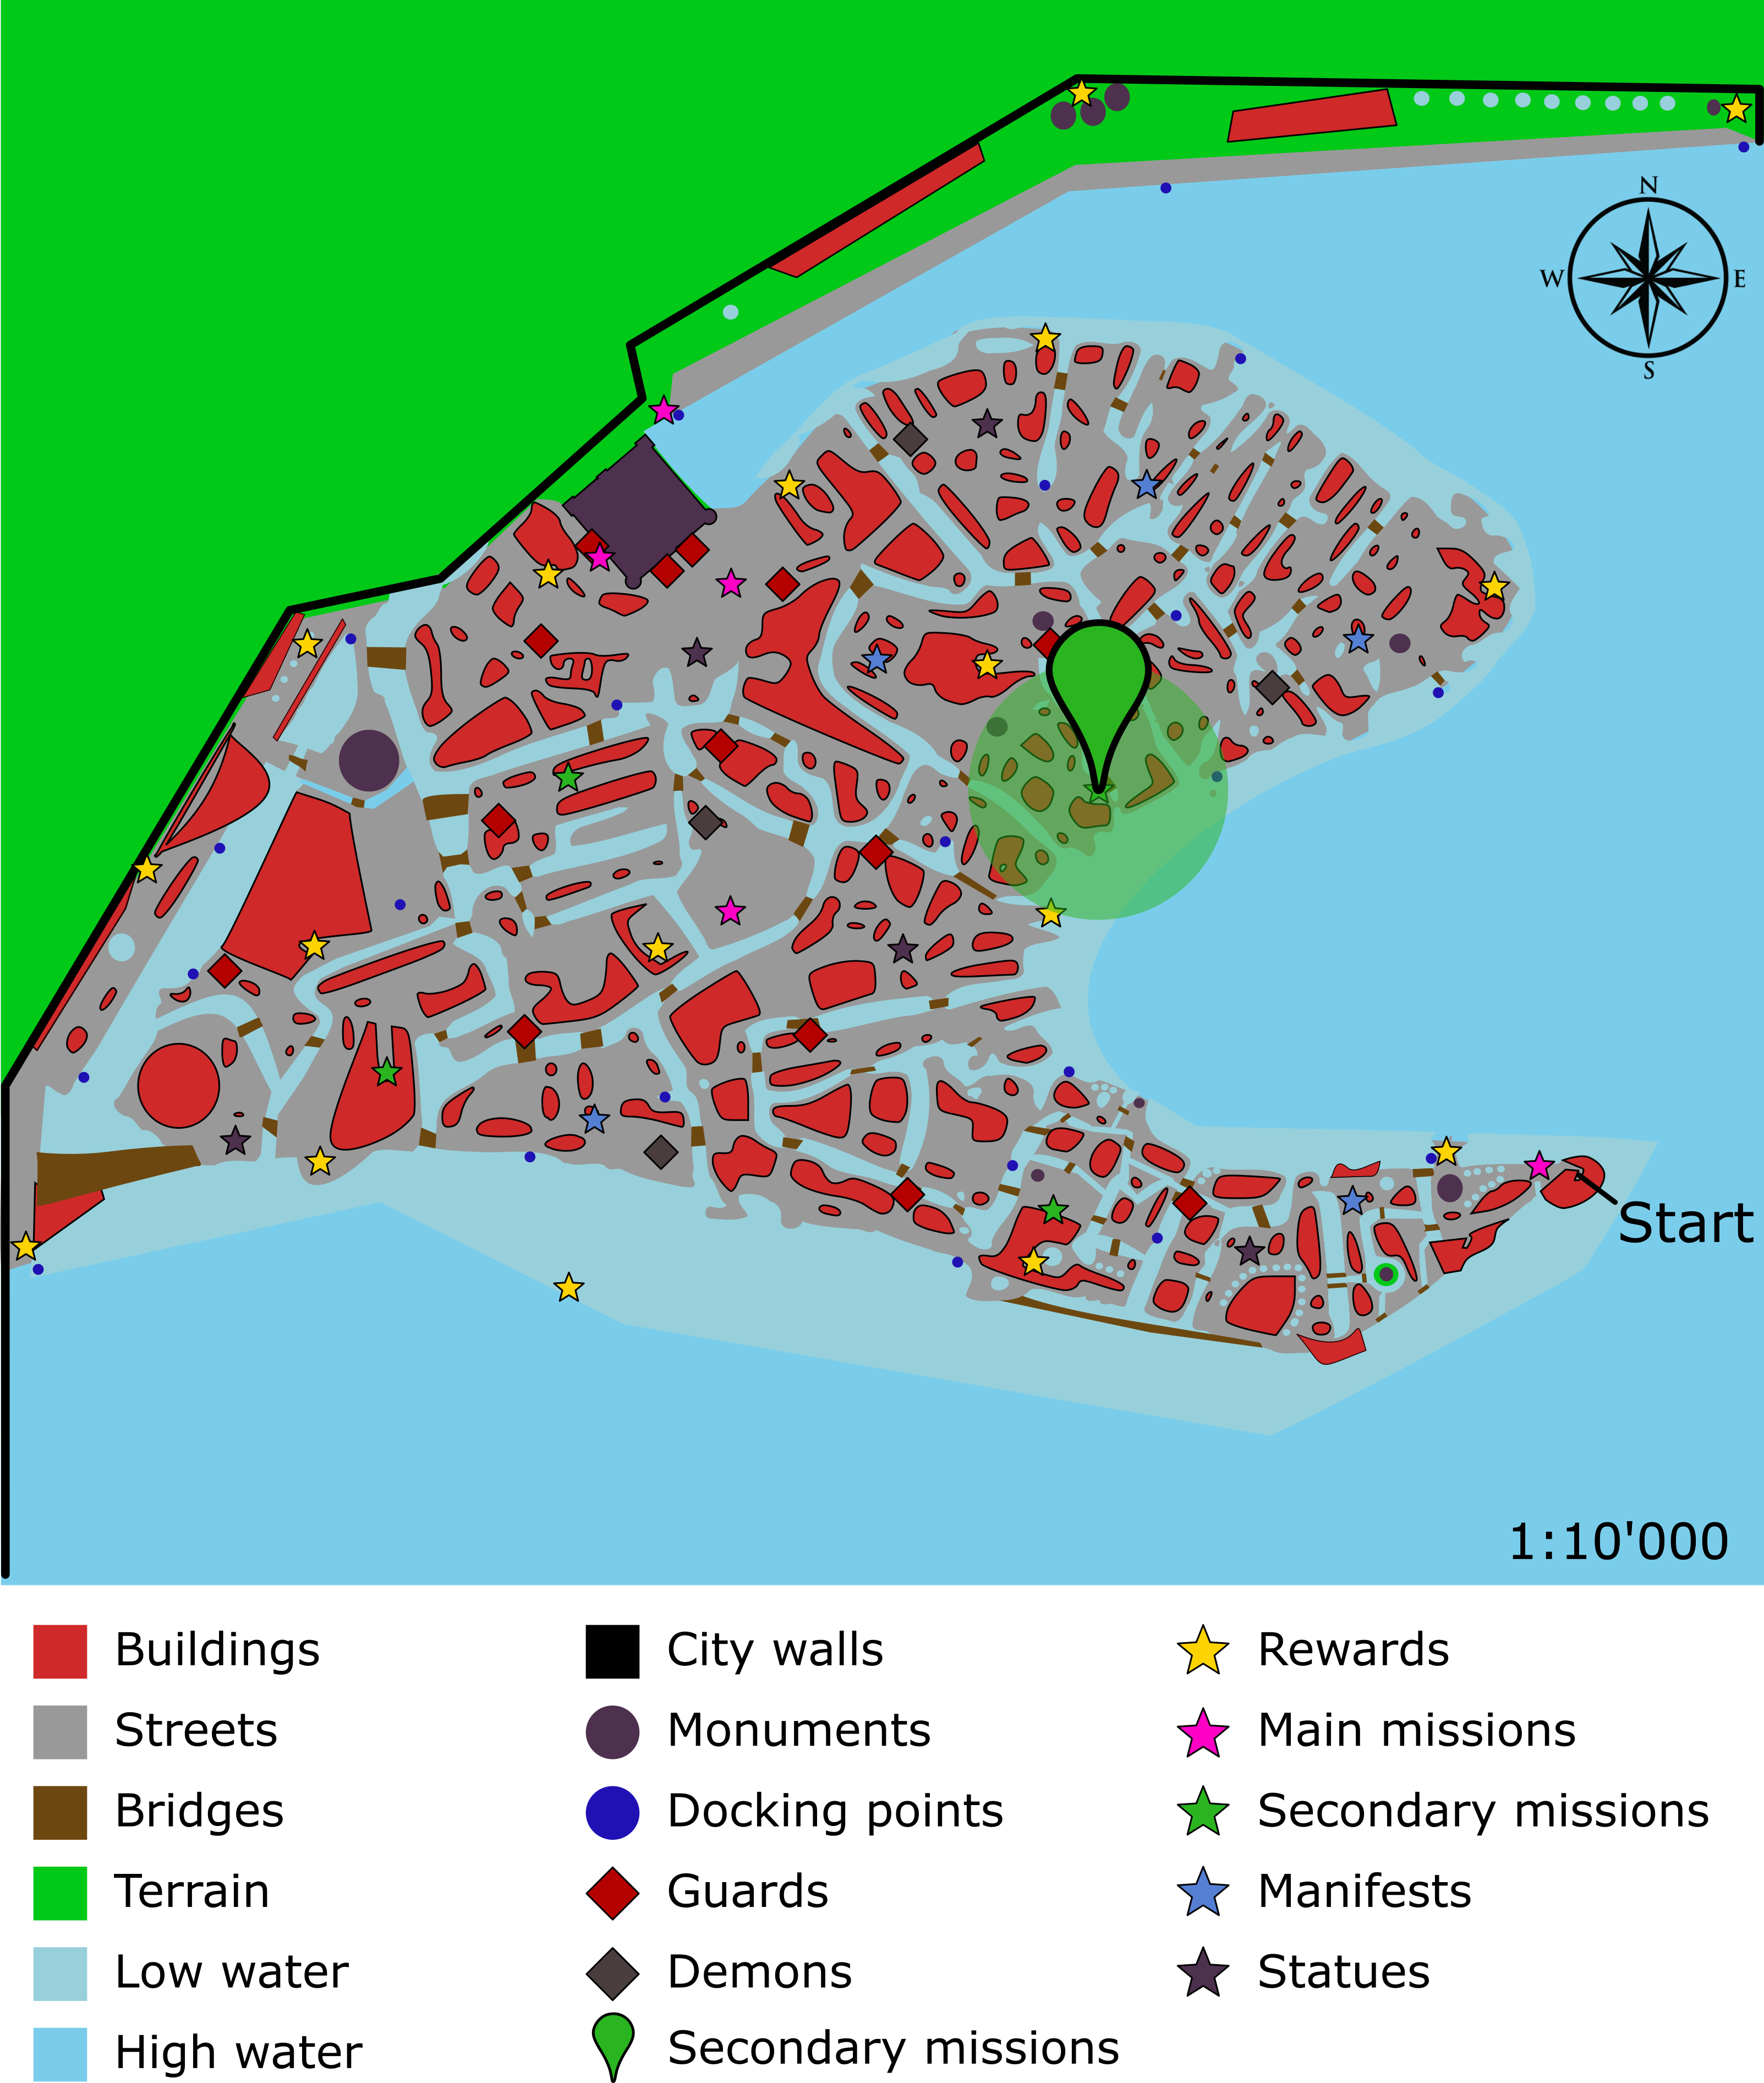
\includegraphics[width=\textwidth]{../Images/Maps/dynamiaSecondaryMissions_Bridge}
  \caption{Secondary mission initial location and activation area}
\end{figure}

\subsubsection*{Starting mission cutscene}
\begin{screenplay}
\extslug[afternoon]{Dynamia, ghetto area}

The tall woman is working on some planks of wood.

\begin{dialogue}{Sophie}
Excuse me, do you need help?
\end{dialogue}

\begin{dialogue}{Tall woman}
Oh, you can bet!
\end{dialogue}

The tall woman stops working to point the collapsed bridge.

\begin{dialogue}[continuing]{Tall woman}
The bridge is collapsed a week ago and nobody did anything. I asked the guards to repair it, but they replied they are too busy.
\end{dialogue}

The tall woman shrugs with resignation.

\begin{dialogue}[continuing]{Tall woman}
No wonder, we are the ghetto after all.
\end{dialogue}

The tall man goes back to working.

\begin{dialogue}{Sophie}
Calcifer, can you do something?
\end{dialogue}

\begin{dialogue}{Calcifer}
I think so, but I need some debris.
\end{dialogue}

\begin{dialogue}{Sophie}
Ok, let's find some.
\end{dialogue}

\end{screenplay}

\subsubsection*{NPC's lines during the mission}
\textbf{Tall woman (busy)}: If you wanna help us, we'll be very grateful.

\subsubsection*{Ending mission cutscene}
\begin{screenplay}
\extslug[afternoon]{Dynamia, ghetto area}

Calcifer uses the collected debris to build a new bridge.

\begin{dialogue}[excited]{Tall man}
Oh, you are amazing! Thank you! Thank you very much! Here. Take this. You've earned it!
\end{dialogue}

%The tall woman gives Sophie TODO.

\end{screenplay}

\subsubsection*{NPC's lines after the mission}
\textbf{Tall woman}: You're really a kind girl. I wish you well.



\subsection{Help the dissident councilman}
Help a dissident councilman to reach a specific docking point in the harbor and take a boat to leave Dynamia before the guards get him.

While in the harbor area, the player can hear the voice of the councilman asking from help from a small dead end.

The councilman's boat is guarded by a guard. The player can use Calcifer's ranged attack to destroy a support as a diversion to trick the guard, or he/she can fight him.

The councilman is a 50-years-old fat man. He wears expensive clothes, but he is sweaty and looks messy. He often uses an embroidered silk handkerchief to wipe the sweat.

\textbf{Reward}: 300 coins, 150 Exp.

\begin{figure}[H]
  \centering
  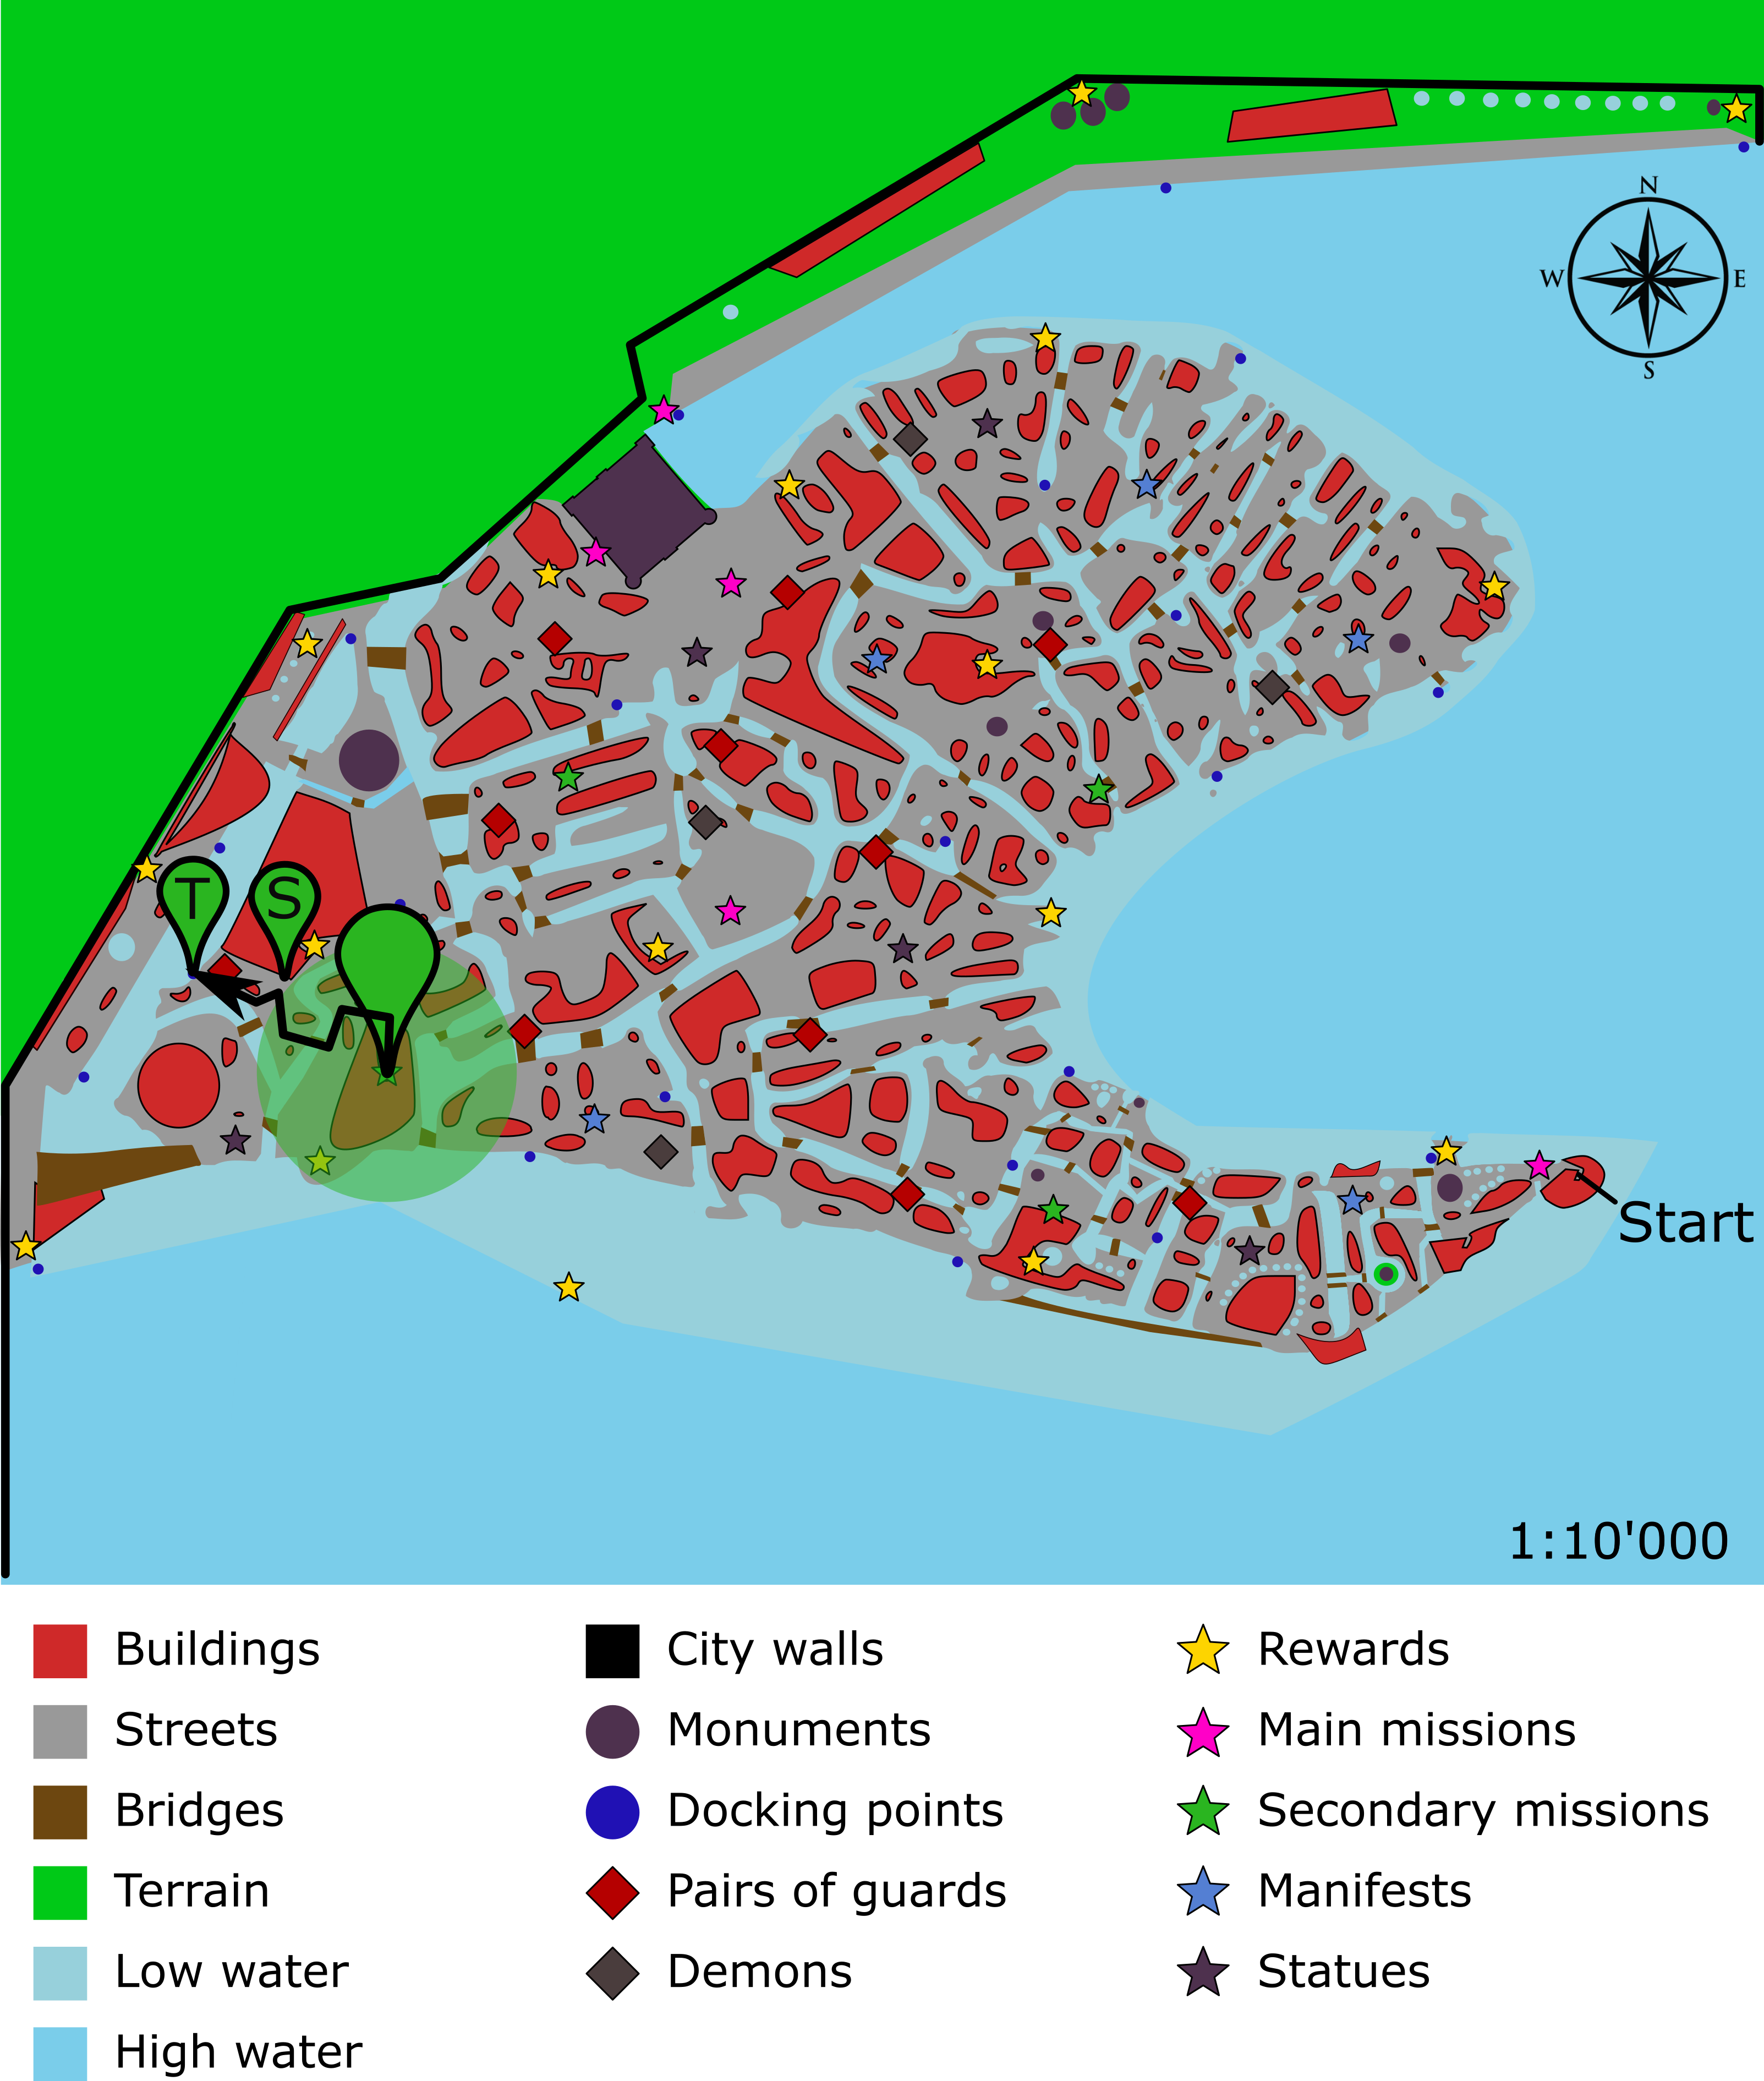
\includegraphics[width=\textwidth]{../Images/Maps/dynamiaSecondaryMissions_Councilman}
  \caption{Secondary mission initial location, activation area, target location (T) and support location (S)}
\end{figure}

\subsubsection*{Starting mission cutscene}
\begin{screenplay}
\extslug[afternoon]{Dynamia, harbor area}

A demon has trapped a scared fat man in a dead end. The demon is getting closer to the man.

\begin{dialogue}{Sophie}
Calcifer!
\end{dialogue}

Calcifer attacks the demon, that runs away.

\begin{dialogue}[grateful]{Councilman}
My savior! You saved my life!
\end{dialogue}

\begin{dialogue}{Sophie}
Why has it attacked you?
\end{dialogue}

The councilman uses his silk handkerchief to wipe the sweat and looks around worried.

\begin{dialogue}[at low voice]{Councilman}
The queen wants me dead. She's hunting all the councilmen who had not supported her coronation. I KNEW there is something wrong with her. May I ask your help again? I need to reach the dock number two. Please, I can pay you.
\end{dialogue}

\end{screenplay}

\textit{\textbf{CHOICE}}
\begin{itemize}
\item \textbf{Accept the mission}

\begin{screenplay}

\begin{dialogue}{Sophie}
Ok, let's go.
\end{dialogue}

\begin{dialogue}[grateful]{Councilman}
You're an angel, miss! Thank you very much!
\end{dialogue}

\end{screenplay}

\item \textbf{Decline the mission}

\begin{screenplay}

\begin{dialogue}{Sophie}
I'm sorry, I really have to go.
\end{dialogue}

\begin{dialogue}[disappointed]{Councilman}
Oh, I see. Anyway, thank you for saving my life. I'll stay nearby, it's too dangerous to move around right now.
\end{dialogue}

\end{screenplay}

\end{itemize}

If the player declines the mission, he/she can talk again to the councilman and accept the mission:

\hspace{1em} \textbf{Councilman}: Please, I need to reach the dock number two. I can pay you.

\hspace{1em} The player will be asked again for the same choice as before.

\subsubsection*{NPC's lines during the mission}
\textbf{Councilman (scared)}: I need to reach the dock number two. A boat is waiting there for me.

\subsubsection*{Support cutscene (when the player sees the guard)}
\begin{screenplay}
\extslug[afternoon]{Dynamia, harbor area}

A guard is patrolling the area in front of the councilman's boat. Sophie and the councilman hide behind a wall before being spotted.

\begin{dialogue}[worried]{Councilman}
Oh, no, that's my boat. What can we do now?
\end{dialogue}

\begin{dialogue}{Calcifer}
Don't worry, it's just a guard. We can handle it!
\end{dialogue}

Sophie looks around and sees the support.

\begin{dialogue}{Sophie}
Well, maybe we don't have to fight.
\end{dialogue}

\end{screenplay}

\subsubsection*{Ending mission cutscene}
\begin{screenplay}
\extslug[afternoon]{Dynamia, harbor area}

The councilman shakes Sophie's hand.

\begin{dialogue}[grateful]{Councilman}
You really did it, miss. As promised, here is your reward.
\end{dialogue}

The councilman pays Sophie.

\begin{dialogue}[continuing]{Councilman}
The boat is waiting for me. Thank you again.
\end{dialogue}

The councilman gets on the boat and the boat leaves.

\end{screenplay}


\subsection{Defeat all the enemies in the Castle}
Defeat all the guards, the demons and the captain inside the Castle of Dynamia. In order to do that, the player has to ignore the puzzles.

This mission is alternative to \textit{Avoid all the enemies in the Castle}.

\textbf{Reward}: 500 Exp.

\subsection{Avoid all the enemies in the Castle}
Avoid all the guards, the demons and the captain inside the Castle of Dynamia. In order to do that, the player has to focus on solving the puzzles.

This mission is alternative to \textit{Defeat all the enemies in the Castle}.

\textbf{Reward}: 500 Exp.


%\subsection{Find all the writings on the wall in the Castle}
%Find all the writings on the wall in the Castle.
%
%Some writings are placed in rooms patrolled by the enemies or hidden in the secret passages, so the player has to fight the enemies and solve the puzzles in order to find them all.
%
%\textbf{Reward}: TODO Exp.
%
%TODO: write down all the writings.
